% ---------------------------------------------------------------------------
% Paper 01 -- Obstruction certificates for viability under incomplete observation
% Edition v73 (research-article rewrite of v72; see CHANGELOG_v72_to_v73.md)
% Build: tectonic paper01_obstruction_calculus_v73.tex
% ---------------------------------------------------------------------------
\documentclass[11pt,a4paper]{article}
\usepackage[a4paper,margin=26mm]{geometry}
\usepackage[T1]{fontenc}
\usepackage{lmodern}
\usepackage{microtype}
\usepackage{amsmath,amssymb,amsthm}
\usepackage{graphicx}
\graphicspath{{./}{paper01_obstruction_calculus_v73_src/}}
\usepackage{booktabs,array,tabularx,multirow}
\usepackage[font=small,labelfont=bf]{caption}
\usepackage[round,authoryear]{natbib}
\usepackage{enumitem}
\usepackage[colorlinks=true,linkcolor=blue!50!black,citecolor=blue!50!black,urlcolor=blue!50!black]{hyperref}
\usepackage{etoolbox}
\usepackage{xcolor}
\setlength{\bibsep}{3pt plus 1pt}
\allowdisplaybreaks
\emergencystretch=2em

% ---- theorem environments: one counter per section
\theoremstyle{plain}
\newtheorem{theorem}{Theorem}[section]
\newtheorem{proposition}[theorem]{Proposition}
\newtheorem{corollary}[theorem]{Corollary}
\newtheorem{lemma}[theorem]{Lemma}
\theoremstyle{definition}
\newtheorem{definition}[theorem]{Definition}
\newtheorem{example}[theorem]{Example}
\newtheorem{openproblem}[theorem]{Open Problem}
\theoremstyle{remark}
\newtheorem{remark}[theorem]{Remark}

% ---- macros
\newcommand{\R}{\mathbb{R}}
\newcommand{\Viab}{\mathrm{Viab}}
\newcommand{\RViab}{\mathrm{RViab}}
\newcommand{\ERViab}{\mathrm{ERViab}}
\newcommand{\EViab}{\mathrm{EViab}}
\newcommand{\IRViab}{\mathrm{IRViab}}
\newcommand{\cV}{\mathcal{V}}
\newcommand{\cI}{\mathcal{I}}
\newcommand{\cJ}{\mathcal{J}}
\newcommand{\cR}{\mathcal{R}}
\newcommand{\cA}{\mathcal{A}}
\newcommand{\cW}{\mathcal{W}}
\newcommand{\cY}{\mathcal{Y}}
\newcommand{\cS}{\mathcal{S}}
\newcommand{\Post}{\mathrm{Post}}
\newcommand{\Pre}{\mathrm{Pre}}
\newcommand{\Tobs}{T_{\mathrm{obs}}}
\newcommand{\Atube}{\cA_{\mathrm{tube}}}
\newcommand{\Reach}{\mathrm{Reach}}
\newcommand{\supp}{\mathrm{supp}}
\newcommand{\co}{\operatorname{co}}
\newcommand{\dd}{\,\mathrm{d}}
\newcommand{\hyp}[1]{\textup{(#1)}}

\title{\vspace{-1.2em}Obstruction certificates for viability under incomplete observation\\[0.3em]
{\large A calculus of sufficient conditions for nonviability, with exact finite and polyhedral cases}}
\author{Amin Abaee\\[0.3em]
{\normalsize Independent Researcher}\\
{\normalsize \href{https://orcid.org/0000-0002-0019-1842}{ORCID 0000-0002-0019-1842}\ \ $\cdot$\ \ \href{mailto:amin_abaee@ut.ac.ir}{amin\_abaee@ut.ac.ir}}}
\date{Edition v73 --- October 2026}

\begin{document}
\maketitle
\vspace{-1.5em}
\begin{center}\small\emph{Author preprint, not yet refereed; an earlier edition is deposited at Zenodo and figshare \citep{abaee2026preprint}. The Supplementary Material (Sections S1--S9) carries the complete proofs, worked certificates, the probabilistic counterpart, and the verification record.}\end{center}

\begin{abstract}
\noindent
Under perfect measurement the viability kernel of a constrained control system is characterised by tangency conditions, and under incomplete observation the \emph{sufficiency} side of the theory is served by output-feedback regulation conditions and estimation-tube reductions. The complementary task---certifying that \emph{no} observation-based policy can keep the system within its constraints---has no comparable instrument. This paper develops one: a calculus of \emph{obstruction certificates}, each a checkable witness that a prescribed class of observation-based policies fails because the information structure leaves no room for any policy. The calculus is organised by a single selector principle: an observation-based regulator must choose one response for an entire information state, and viability requires that response to be admissible, safe over the review, and recursively viable for every compatible state. Each certificate proves that one of these response correspondences is empty. The central result, the common-action obstruction, shows that disjoint safe-control sets of states merged by the observation exclude every policy of a held-action class, even when each state is viable under full information; it has a Farkas-pair witness for polyhedral data and a Helly-type sparse witness of at most $m+1$ states for $m$ controls. A delayed-information obstruction turns the timing of the first informative observation into an explicit bound, exactly computable as a linear programme over polytope-declared blind-window classes, and a recourse obstruction certifies the complementary failure of post-observation authority in affine systems. In finite systems the calculus is exact: belief recursion is sound and complete and the common-action test is necessary and sufficient one step ahead. The limits of completeness are made precise---static observation reduces to open-loop robust viability, and no certificate pair that reads only the blind window can be complete. A separate certification layer shows that an exact observation-only safety verdict exists if and only if safe-set membership is constant on the observation fibres. The certificates are instantiated on a symbolic resource model, audited against the exact recursion, and read as design requirements on monitoring timing, coarseness, aggregation and bias. The discrete core is machine-checked in Lean~4.
\end{abstract}

\noindent\textbf{Keywords:} viability kernel; incomplete observation; obstruction certificates; robust viability; output feedback; set-membership estimation; monitoring design; sustainability governance

\smallskip\noindent\textbf{MSC 2020:} 49J53; 93B03; 93C41; 91B76

\section{Introduction}\label{sec:intro}

Viability theory asks from which states of a constrained control system at least one control can keep every future state inside a constraint set \citep{aubin1991}. For sustainability problems the constraints are floors---stock levels, service thresholds, safety margins---and viability is the formal counterpart of maintaining a development path rather than optimising it \citep{bene2001,delara2008,doyen2012,doyen2020}. Under \emph{perfect measurement} the theory is complete in the relevant sense: the viability kernel exists as the largest viable subset of the constraint set, Nagumo-type tangency conditions characterise it, and approximation schemes compute it \citep{saintpierre1994,aubin2011}.

Sustainability governance, however, operates under \emph{incomplete observation}. Stocks are assessed at discrete review intervals; indicators are coarser than the state; some stocks are not observed at all; and the information that does arrive may arrive late. The signal that would reveal an erosion of the productive base is often precisely the one that is coarse, postponed, or absent, because a base can be drawn down while the measured output is held up. Incomplete observation is therefore structural to the certification problem, not a practical nuisance.

The viability question under incomplete observation splits into two directions. The sufficiency direction has a canonical literature. \citet{veliov1993} gives conditions for the existence of an output-feedback regulation map under incomplete and inexact measurement, reducing under perfect measurement to the classical viability condition of \citet{haddad1981}; the estimation-tube programme absorbs imperfect measurement into set-valued dynamics on a space of sets of compatible states \citep{kurzhanski1997,cardaliaguet2007}; barrier certificates certify safety from a scalar function \citep{prajna2004,prajna2007}, with converse and hybrid characterisations \citep{prajna2005,maghenem2019}; and Hamilton--Jacobi reachability computes backward reachable tubes as sublevel sets of viscosity solutions \citep{mitchell2005,margellos2011,bansal2017}. All of these are, in direction, sufficiency machines: they compute or certify the states from which some control preserves safety.

What that literature does not supply is the converse instrument: a systematic way of \emph{certifying that no observation-based policy is viable}, and of saying which feature of the observation design---its timing, coarseness, aggregation or bias---is responsible. This paper develops that instrument. An \emph{obstruction certificate} is a checkable witness that a prescribed class of observation-based policies fails, not because a particular policy is bad, but because the information structure leaves no room for any policy. Its negation is a necessary condition for observation-based viability. In the polyhedral and finite cases the certificate is a finite object---a Farkas pair, a short list of incompatible states, an obstruction tree---and in the analytic cases it is an explicit adverse trajectory together with a quantitative bound.

\paragraph{The organising idea.} An observation-based regulator cannot tailor its action to the true state; it must select a single response---a held command, a blind-window control, or a safe/unsafe verdict---for an entire information state. Observation-based viability is therefore the existence of one response that is simultaneously admissible, safe until the next observation, and recursively viable, for every state compatible with the record (the \emph{selector principle}, Proposition~\ref{prop:selector}). Each certificate of the paper proves that one of these response correspondences is empty, and the certificates are nested in a ladder. This single viewpoint turns a list of nonviability conditions into a calculus: the mechanism that fires identifies the correspondence that failed, and the correspondence that failed identifies the design change that could restore it.

\paragraph{Contributions.} The paper establishes the following, each stated with the policy class and the hypotheses under which it holds.
\begin{enumerate}[leftmargin=2em,itemsep=2pt]
\item \emph{Exactness in finite systems} (Section~\ref{sec:finite}). Backward recursion over set-valued beliefs is sound and complete on every finite horizon (Theorem~\ref{thm:finite-horizon}), and one step ahead the common-action test is necessary and sufficient (Theorem~\ref{thm:onestep}); nonviability is witnessed by a finite obstruction tree. This fragment is machine-checked in Lean~4.
\item \emph{The common-action obstruction} (Theorem~\ref{thm:common-action}). At a post-observation information state of a held-action review class, emptiness of the common safe-action set---under a compatible adverse-path hypothesis---excludes every policy, even when each compatible state is viable under full information. For polyhedral data the witness is a Farkas pair; for control-affine dynamics with convex control sets a Helly-type argument bounds the witness by $m+1$ compatible states (Proposition~\ref{prop:helly}). The rungs of the obstruction ladder (Proposition~\ref{prop:ladder}) are the admissibility, safe-action and review-tube correspondences.
\item \emph{The delayed-information obstruction} (Theorem~\ref{thm:delayed}). When the first branch-discriminating observation arrives at time $\Tobs$ and an adverse realisation drives a constraint margin down at rate $\varepsilon$, the explicit bound $\inf q/\varepsilon<\Tobs$ excludes every policy of the blind-window class; the bound has a sharp threshold form (Remark~\ref{rem:sigma}), and over polytope-declared blind-window classes the threshold is exactly computable as a linear programme whose Farkas dual is the certificate (Theorem~\ref{thm:lp}). The class declaration is load-bearing: a whole-window hold class can have an unbounded survival gap relative to its per-step polytope relaxation (Example~\ref{ex:relax-gap}).
\item \emph{Dynamic and recourse obstructions} (Theorem~\ref{thm:exit}, Proposition~\ref{prop:recourse}). A finite-time exit certificate of comparison type closes the viability question before any observation argument, and an oracle-recourse certificate for affine systems detects the complementary mode in which a blind window is survivable but no post-observation authority can recover every branch; a planar braking instance has an exact delay threshold $\tau^*=7/50$ and is genuinely three-way.
\item \emph{Certification limits} (Section~\ref{sec:certification}). An exact observation-only safety certifier exists if and only if safe-set membership is constant on the observation fibres (Proposition~\ref{prop:fibre}); the certainly-safe set is the sound relaxation (Corollary~\ref{cor:certainly-safe}); and a certainty-equivalence controller applied to a biased but injective observation can have an empty kernel while a corrected controller is viable (Proposition~\ref{prop:ce-trap}).
\item \emph{The limits of completeness} (Section~\ref{sec:completeness}). Static observation reduces exactly to open-loop robust viability (Theorem~\ref{thm:static}); the two-phase (blind window, then reveal) problem decomposes exactly (Proposition~\ref{prop:decomposition}); and no certificate pair that reads only the window sub-model can be complete (Proposition~\ref{prop:window-nogo}). The residual dynamic gap is stated as an open problem with a definite target.
\end{enumerate}
The certificates are instantiated on a symbolic resource model and audited, cell by cell, against the exact recursion (Section~\ref{sec:casestudy}); their monitoring and institutional consequences---timing, coarseness, aggregation and bias---are drawn in Section~\ref{sec:discussion}.

\paragraph{Related work.} The nearest neighbour of the question posed here is \citet{doyen2000}, who characterises \emph{guaranteed viability domains} under output feedback: a closed set $K$ is such a domain when there is a Lipschitz selection $u(\cdot)$ of the control constraint map with $K$ invariant under $\dot x\in\{f(x,u(h(x,w)),w):w\in W(x)\}$, and the characterisation is an equivalence whose constructive content is a feedback synthesis by Steiner selection. The present work differs on three axes visible in that statement: the policy class (memoryless Lipschitz functions of the current output there; measurable nonanticipative functions of the whole record here), the property (exact invariance of a closed set there; viability of information states here), and the direction---the obstruction side, which \citet{doyen2000} records as undeveloped (``no general viability result is available in this differential game context with imperfect and/or partial information''). On the failure side under full information, \citet{aubin2001} characterises the complement of the kernel together with capture basins, and \citet{aubin2002} supply the bilateral-fixed-point calculus; the certificates below are one-sided, observation-constrained analogues of that programme. Robust viability is \citet{aubinfrankowska1990} and \citet{frankowska1989}; viability with observable parameters is \citet{quincampoix1994}. The set-membership information state used throughout is that of \citet{kurzhanski1997}; the finite belief recursion is the set-valued analogue of the belief-state recursion of partially observable Markov processes \citep{astrom1965,smallwood1973}, whose qualitative safety variant is \citet{chatterjee2009}, and whose complexity is \citet{papadimitriou1987}. Hamilton--Jacobi reachability \citep{mitchell2005,margellos2011,bansal2017}, resting on viscosity-solution theory \citep{crandall1992}, indexes its value by a physical state, whereas this paper tracks sets of compatible states; its learning-based extensions \citep{bansal2021} purchase scalability with approximation. Shield-based runtime enforcement for finite stochastic models \citep{alshiekh2018} restricts an arbitrary policy to precomputed safe actions and is a sufficiency device in the present sense. A companion robust-viability application to a fishery limit reference point is \citet{abaee2026fish}, and the minimax-dual development of the common-action witnesses is a separate companion manuscript \citep{abaee2026minimax}. To the author's knowledge the common-action and delayed-information obstructions and the fibre criterion have not been stated in this form; the elementary facts on which they rest---quantifier commutation, Dini comparison, Farkas' lemma and Helly's theorem---are classical.

\paragraph{Organisation.} Section~\ref{sec:setting} fixes the setting, consolidates the standing conventions, and states the selector principle. Section~\ref{sec:finite} treats finite systems, where the calculus is exact. Section~\ref{sec:calculus} develops the continuous-time certificates. Section~\ref{sec:certification} treats certification limits, Section~\ref{sec:completeness} the limits of completeness, Section~\ref{sec:casestudy} the worked model and coverage audit, and Section~\ref{sec:discussion} the position of the calculus and its design consequences. Short proofs are given in place; complete proofs of the longer statements, the worked certificates, the probabilistic counterpart, the expanded review of the sufficiency literature, and the verification record are in the Supplementary Material (cited as S1--S9). Table~S9.1 maps every result of this edition to its predecessor.
\section{Setting, conventions, and the selector principle}\label{sec:setting}

\subsection{Dynamics, constraints, and the kernel hierarchy}\label{sec:kernels}

Fix a state space $X\subseteq\R^n$, a control set $U$, a disturbance set $D$, and dynamics
\begin{equation}\label{eq:dyn}
\dot x(t)=f\bigl(x(t),u(t),d(t)\bigr),\qquad u(t)\in U(x(t)),\quad d(t)\in D(x(t)),
\end{equation}
with $f$ continuous, $U$ and $D$ set-valued with closed graph and nonempty compact values, and admissible controls and disturbances measurable selections. These are the \emph{standing solution-existence conditions}: every selection pair admits a Carath\'eodory solution, and the convexified relaxed inclusion satisfies the Marchaud conditions of the viability literature \citep{aubin1991}. They provide a solution for each fixed selection pair; they do \emph{not} by themselves provide an adversarial selection coupled to a policy, which is why the analytic certificates below carry an explicit adverse-path hypothesis. Let $\cV\subseteq X$ be a closed constraint set, described where needed by finitely many $C^1$ functions, $\cV=\{x:q_j(x)\ge0,\ j=1,\dots,m_q\}$. Strict floor violation means $q_j<0$.

Three kernels organise the analysis. $\Viab(\cV)$ is the \emph{viability kernel} under state feedback without disturbance, the largest closed subset of $\cV$ from which some state-feedback control keeps the trajectory in $\cV$ for all time \citep{aubin1991}. $\RViab(\cV)$ is the \emph{robust kernel}, from which some state-feedback policy keeps every trajectory in $\cV$ for every admissible disturbance realisation \citep{aubinfrankowska1990}. The object of this paper is the \emph{robust epistemic kernel} $\ERViab_\cI(\cV)$ (Definition~\ref{def:kernel}), whose elements are \emph{information states}, not physical states. Writing $\mathrm{proj}_\exists(\mathfrak B)=\bigcup_{B\in\mathfrak B}B$ for the existential projection of a collection of information states, the informational hierarchy reads
\begin{equation}\label{eq:hierarchy}
\mathrm{proj}_\exists\bigl(\IRViab_\cJ(\cV)\bigr)\;\subseteq\;\mathrm{proj}_\exists\bigl(\ERViab_\cI(\cV)\bigr)\;\subseteq\;\RViab^{\mathrm{hist}}(\cV),
\end{equation}
where $\IRViab_\cJ(\cV)$ is the \emph{institutionally restricted} kernel---the epistemic kernel with the observations and actions restricted to those an institution $\cJ$ may receive and command (Section~\ref{sec:design})---and $\RViab^{\mathrm{hist}}$ permits nonanticipative full-information histories. Identifying $\RViab^{\mathrm{hist}}$ with the state-feedback kernel requires a comparison theorem matching admissibility, solution and policy classes, and none is assumed. Each inclusion can be strict for a distinct reason: robust contraction arises from disturbances, epistemic contraction from indistinguishability, institutional contraction from restricted authority. This paper characterises the epistemic contraction.

\subsection{Observation structures and information states}\label{sec:information}

An \emph{observation structure} $\cI=(Y,O)$ is a measurable space $Y$ with an observation map $O:X\to Y$; the policy observes $y(t)=O(x(t))$. The \emph{information state} (belief) at time $t$ of a regulator who knows the dynamics, the disturbance class, its own applied controls $(u(s))_{s<t}$ and the record $(y(s))_{s\le t}$ is the set of current states compatible with all of them,
\begin{equation}\label{eq:belief}
B_t=\bigl\{\xi(t):\ \xi(0)\in B_0,\ \dot\xi=f(\xi,u,d),\ d(s)\in D(\xi(s)),\ O(\xi(s))=y(s)\ \forall s\le t\text{ observed}\bigr\},
\end{equation}
the applied control history being the regulator's own and common to every candidate trajectory. This is the set-membership semantics of \citet{kurzhanski1997}. A \emph{prior} $B_0$ is a belief before the initial reading; the initial reading $y_0=O(x_0)$ is available before the first action, so the first decision is taken at the \emph{post-observation cell} $B_{0,y}=B_0\cap O^{-1}(y)$, and every later belief lies in one current observation cell. A policy is \emph{observation-based} when it is a measurable nonanticipative function of the available record; a \emph{belief-based} policy factors through $B_t$ and is a special case. The common admissible action set of a belief is
\[
U^B(B)=\bigcap_{x\in B}U(x),
\]
the only actions an observation-based policy can select without risking inadmissibility at some compatible state.

\begin{definition}[robust epistemic kernel]\label{def:kernel}
$B_0\in\ERViab_\cI(\cV)$ if there exists a nonanticipative observation-based policy $\pi$ such that, for every compatible initial state $x_0\in B_0$ and every admissible disturbance realisation $d(\cdot)$, every trajectory of \eqref{eq:dyn} generated from $x_0$ by $\pi$'s actions under $d(\cdot)$---the record being the one that $(\pi,d(\cdot))$ generates---remains in $\cV$ for all time.
\end{definition}

The quantifier order is the exists-strategy-for-all-realisations form and is essential: the record is generated by the realisation, so conditioning admissible realisations on the record would be circular. The ambient domain is $\mathfrak B=\{B\subseteq X:B\ne\varnothing\}$; compactness of beliefs or fibres is assumed only where a statement needs it. The non-robust counterpart $\EViab_\cI(\cV)$ (some policy and \emph{some} realisation keep every compatible trajectory safe) is a strictly weaker contrast class, and none of the results below transfers to it a fortiori. When $O$ is injective the record determines the state, the informational certificates reduce to the no-merge case, and only the dynamic obstruction can certify exclusion.

\paragraph{Standing conventions.} Four conventions are used throughout and are collected here so that each statement can refer to them by name.
\begin{description}[leftmargin=1.6em,itemsep=1pt]
\item[\hyp{Fail}] An action outside $U(x)$ applied at a compatible state $x$ is itself failure.
\item[\hyp{Hold}] A \emph{held-action review class} selects a command at each review and holds it over the review interval of positive length $\Delta$; within-review switching is excluded. Statements that need this class say so; a continuous record and time-varying controls are otherwise permitted.
\item[\hyp{Record}] Policies are functions of the full nonanticipative record. Representing them by the set-valued belief is justified when the exact belief is a sufficient statistic and a measurable belief-policy selector exists, not by the definition of a record alone.
\item[\hyp{Order}] The disturbance-information order is statement-specific: the common-action and delayed witnesses respond to a candidate policy ($\forall\pi\,\exists d$); the recourse witness is one exogenous scenario admissible against all policies ($\exists d\,\forall\pi$).
\end{description}
Under exact rectangular belief dynamics and a strategy class closed under nonanticipative concatenation, the epistemic kernel is a recursively viable family of information states; without those hypotheses this is an organising description rather than a greatest-fixed-point theorem. Observation error, hidden parameters and delays require their own information models (error: $y\in H(\xi,v)$; parameters: beliefs in $X\times\Theta$; delays: beliefs in a history space) and are noted as extensions in Section~\ref{sec:limitations}.

\subsection{The safe-control correspondence}\label{sec:safecontrol}

For $x\in\cV$ define the \emph{safe-control correspondence}
\begin{equation}\label{eq:R}
\cR_\cV(x)=\bigl\{u\in U(x):\ \forall d\in D(x),\ \forall j\text{ with }q_j(x)=0:\ \nabla q_j(x)\cdot f(x,u,d)\ge0\bigr\},
\end{equation}
the controls whose drift is inward on every active constraint face uniformly over the disturbance; at interior points $\cR_\cV(x)=U(x)$. Two readings must be kept apart. In the \emph{local} reading, the active-gradient inequalities are necessary for a contingent tangent velocity; they are also sufficient only under a representation regularity condition such as the Mangasarian--Fromovitz qualification ($q(x)=x^3$, $\cV=[0,\infty)$ and velocity $-1$ at $0$ satisfy $\nabla q(0)\cdot(-1)=0$ yet exit immediately). By contrast, a \emph{strictly negative} derivative along an admissible original-system path through an active constraint is a local obstruction with no qualification needed. In the \emph{kernel} reading, viability of $x_0\in\cV$ requires a selection in $\cR_G$ along the trajectory with $G=\RViab(\cV)$, since points of $\cV\setminus G$ may admit instantaneously safe controls while every trajectory exits later. The obstruction theorems below are local certificates against $\cR_\cV$: exhibiting a belief at which even the weaker pointwise condition fails, together with a realised exiting path, certifies exclusion from the kernel. The correspondence is the object on which the observation structure acts, through its common value $\cR^B_\cV(B)=\bigcap_{x\in B}\cR_\cV(x)$.

\subsection{Response correspondences and the selector principle}\label{sec:selector}

An observation-based regulator selects a single response for an entire information set. Three response correspondences are used in continuous time:
\begin{align*}
U^B(B)&=\textstyle\bigcap_{x\in B}U(x) &&\text{(admissibility)},\\
\cR^B_\cV(B)&=\textstyle\bigcap_{x\in B}\cR_\cV(x) &&\text{(instantaneous safety)},\\
\Atube(B,\Delta)&=\{a\in U^B(B):\ \mathrm{Safe}_{\mathrm{hold}}(B,a,\Delta)\} &&\text{(review-interval safety)},
\end{align*}
where $\mathrm{Safe}_{\mathrm{hold}}(B,a,\Delta)$ means that every compatible original-system trajectory under the held command $a$ exists, remains in $\cV$, and obeys $a\in U(x(t))$ throughout $[0,\Delta]$, quantified over all compatible initial states, admissible disturbances and solutions. The last condition matters when admissible controls depend on the state: initial common admissibility does not imply trajectory-wise admissibility. In finite systems a fourth, recursive correspondence $\cA_N(B)$ is defined in Section~\ref{sec:finite}. Write $\Reach_{[0,\Delta]}(B,a)$ for the set of states of these held-action trajectories.

\begin{proposition}[selector principle]\label{prop:selector}
Let $B\in\ERViab_\cI(\cV)$ be a post-observation cell of a held-action review class \hyp{Hold} and let $\pi$ witness its viability. Then at every review the action $a=\pi(B)$ is (i) \emph{admissible}, $a\in U^B(B)$; (ii) \emph{safe}, $\Reach_{[0,\Delta]}(B,a)\subseteq\cV$; and (iii) \emph{recursively viable}: every post-observation belief reached at the next review lies again in $\ERViab_\cI(\cV)$ under the continuation of $\pi$. Consequently, along every reachable branch, $U^B(B_k)\ne\varnothing$ and $\Atube(B_k,\Delta)\ne\varnothing$; in the sampled model of Section~\ref{sec:finite} the recursive predecessor is nonempty as well; and $\cR^B_\cV(B_k)\ne\varnothing$ holds under the adverse-path premise \hyp{C3} of Theorem~\ref{thm:common-action} at every failed active-gradient test. A certificate that any one of these correspondences is empty at a reachable belief therefore certifies nonviability under the hypotheses declared for that certificate.
\end{proposition}

\begin{proof}[Proof sketch]
(i) The record through the review is common to the cell and the policy applies one action whatever the compatible true state; inadmissibility at any compatible state is failure by \hyp{Fail}. (ii) Over the review a run of $\pi$ applies the held command, so its review segment is a compatible held-action trajectory, and conversely every such trajectory is the review segment of a run (extend the disturbance selection measurably); all these states lie on runs that $\pi$ keeps in $\cV$. (iii) For $x'$ in a reached belief $B'$, the membership of $x'$ in $B'$ supplies a compatible candidate trajectory over the review; gluing its disturbance selection to any continuation realisation gives a run of $\pi$ from a compatible state whose conditioning at the end of the review is the realised one, and witnessing keeps it in $\cV$. The induction over reviews and the per-correspondence consequences are carried out in S2.1, together with a witness showing that the unconditional gradient clause is \emph{not} provable under the standing assumptions: a closed-graph $D$ may carry point values realised by no admissible trajectory, and where only such phantom values fail the gradient test, $\cR^B_\cV(B)=\varnothing$ can coexist with viability.
\end{proof}

The selector principle is the organising claim of the calculus and is used implicitly by every certificate of Sections~\ref{sec:calculus} and \ref{sec:certification}. In finite systems its converse is exact (Theorem~\ref{thm:finite-horizon}); in continuous time no general finite backward-recursion converse is claimed (Section~\ref{sec:completeness}).

\paragraph{Notation.} $\cI$ is always the observation structure and $\cJ$ the institution. $\Tobs$ is the first time the record discriminates between compatible branches. $D^+q(x;v)=\limsup_{h\downarrow0}[q(x+hv)-q(x)]/h$ is the upper right Dini derivative, equal to $\nabla q(x)\cdot v$ for $C^1$ $q$. $h_U(g)=\sup_{v\in U}g^\top v$ is the support function of $U$. A few letters carry local meanings declared where they occur: $a$ is a held action, and also the strip width of Theorem~\ref{thm:exit}; $\lambda$ and $\mu$ are Farkas multipliers or pooling weights; $K$ is the safe set of Section~\ref{sec:certification} and the blind-window length of Theorem~\ref{thm:lp}. The companion manuscripts of this programme share this vocabulary; a concordance of letters whose meanings differ across them is given in S1.
\section{Finite systems: an exact calculus}\label{sec:finite}

In the finite setting the calculus is complete, and the finite statements fix the shape that the continuous certificates approximate. Fix finite state, action, disturbance and observation spaces $X,A,D,Y$, a transition map $x^+=F(x,a,d)$, an observation map $y=O(x,a,d,x^+)$, a safe set $\cV\subseteq X$, and admissible-action sets $U(x)\subseteq A$. For a post-observation belief $B\subseteq X$ contained in one observation cell, an action $a$ and a successor observation $y$, the \emph{post-belief} is
\[
\Post(B,a,y)=\bigl\{x^+\in X:\ \exists\,x\in B,\ d\in D(x),\ x^+=F(x,a,d),\ y=O(x,a,d,x^+)\bigr\},
\]
and $y$ is \emph{possible} under $(B,a)$ if $\Post(B,a,y)\ne\varnothing$. The one-step predecessor of a collection $\mathcal C$ of beliefs is
\[
\Pre(\mathcal C)=\bigl\{B\subseteq\cV:\ \exists\,a\in U^B(B)\ \text{with}\ \Post(B,a,y)\in\mathcal C\ \text{for every possible }y\bigr\},
\]
and the finite-horizon kernels are $\cW_0=\{B:B\subseteq\cV\}$, $\cW_{k+1}=\Pre(\cW_k)$. The $N$-step \emph{recursive witness set} of a belief is $\cA_N(B)=\{a\in U^B(B):\Post(B,a,y)\in\cW_{N-1}\text{ for every possible }y\}$, so that $B\in\cW_N$ iff $\cA_N(B)\ne\varnothing$; this is the fourth, recursive response correspondence of the selector principle.

\begin{theorem}[finite-horizon soundness and completeness]\label{thm:finite-horizon}
A post-observation cell $B_0$ admits an observation-based policy keeping every compatible trajectory in $\cV$ for $N$ steps if and only if $B_0\in\cW_N$. A prior $P\in\mathfrak B$ is $N$-step viable if and only if every nonempty cell $P\cap O^{-1}(y)$ belongs to $\cW_N$.
\end{theorem}

\begin{proof}
The initial reading partitions a prior into disjoint cells on which one policy may choose independently, so the post-observation statement suffices. ($\Rightarrow$) Induction on $N$; the case $N=0$ is $B_0\subseteq\cV$. A policy safe for $N$ steps plays a first action admissible at every compatible state, so $a\in U^B(B_0)$, and for every possible $y$ the successor belief $\Post(B_0,a,y)$ is safe for $N-1$ steps under the same policy, hence lies in $\cW_{N-1}$ by induction; so $B_0\in\Pre(\cW_{N-1})$. ($\Leftarrow$) Backward induction: from $B_k\in\cW_{N-k}$ choose a witness action $a_k\in\cA_{N-k}(B_k)$; after the observation $y_k$ the belief $\Post(B_k,a_k,y_k)$ lies in $\cW_{N-k-1}$, and every reachable state over $N$ steps lies in $\cV$.
\end{proof}

If $B_0\notin\cW_N$ the failure is certified by a finite \emph{obstruction tree}: at each node $(B,k)$ with $k\ge1$ and each $a\in U^B(B)$ the adversary selects a possible observation $y$ with $\Post(B,a,y)\notin\cW_{k-1}$, the tree alternating regulator and nature turns as in partial-information games (S2.2, Figure~S8.2). The recursion is exact but of worst-case complexity exponential in $|X|$, since the belief space has up to $2^{|X|}$ members; finite checkability is per belief, not a polynomial-time global procedure.

\begin{theorem}[one-step completeness]\label{thm:onestep}
Let $S_1(x)=\{a\in U(x):F(x,a,d)\in\cV\ \text{for all }d\in D(x)\}$ be the one-step safe set. A post-observation cell $B\subseteq\cV$ is one-step viable under $\cI$---some observation-based policy achieves $x_1\in\cV$ for every $x_0\in B$ and every admissible disturbance---if and only if $\bigcap_{x\in B}S_1(x)\ne\varnothing$. Hence $B\notin\cW_1$ exactly when the common safe-action set is empty.
\end{theorem}

\begin{proof}
($\Rightarrow$) Every $x\in B$ produced the same record, so the policy plays a single $a\in U^B(B)$, and first-step safety forces $F(x,a,d)\in\cV$ for all $x\in B$ and $d\in D(x)$, i.e.\ $a\in\bigcap_{x\in B}S_1(x)$. ($\Leftarrow$) Any $a$ in the intersection keeps every successor in $\cV$.
\end{proof}

Combined with the recursion $\cW_{k+1}=\Pre(\cW_k)$, Theorem~\ref{thm:onestep} shows that the pair \emph{(common-action test, recursion)} is a complete characterisation at every finite horizon in finite systems: the test detects first-step emptiness and the recursion propagates the obstruction. The common-action test is the discrete form of the central continuous certificate (Theorem~\ref{thm:common-action}).

\begin{example}[hidden-mode conflict]\label{ex:hidden-mode}
An unobserved mode $\theta\in\{-1,+1\}$ drives $z^+=z+\theta u$ on $z\in\{-1,0,1\}$ with $u\in\{-1,+1\}$, safe set $\{z\ge0\}$ and observation $O(z,\theta)=z$. At the belief $B_0=\{(0,-1),(0,+1)\}$ both actions are admissible, but under $u=+1$ the branch $\theta=-1$ reaches $z=-1$ and under $u=-1$ the branch $\theta=+1$ does; so $\bigcap S_1=\varnothing$ and $B_0\notin\cW_1$, although each mode is viable on its own (play $u=\theta$). The obstruction tree is a root with two adversary edges, one per mode. This is the two-action skeleton of every ``the stock is either recovering or collapsing, and the safe policy differs between the two'' situation, and the failure is purely informational: no stochasticity and no estimation error is involved.
\end{example}

\paragraph{Mechanised verification.} The finite fragment---the predecessor recursion and its monotonicity, Theorem~\ref{thm:finite-horizon} in both directions (completeness returning a history-dependent policy tree), the one-step characterisation, a coinductive infinite-horizon kernel \texttt{EpiK} on which the finite common-action obstruction is proved, the fibre criterion of Section~\ref{sec:certification}, the monotonicity of the finite kernel in admissible actions and disturbances, a perturbed Farkas lemma, and Example~\ref{ex:hidden-mode}---is formalised in Lean~4 in the module \texttt{Formalizations/P1\_Obstruction}, which imports only the project prelude: 33 theorems and 25 definitions, with no \texttt{sorry}, and axiom footprints restricted to Lean's classical axioms. The continuous-time statements of Sections~\ref{sec:calculus}--\ref{sec:completeness} are \emph{not} formalised; they rest on the displayed proofs. Scope, declaration map and build provenance are recorded in S7.
\section{The obstruction calculus in continuous time}\label{sec:calculus}

The continuous-time certificates are sound sufficient conditions for nonviability, each attached to a declared policy class and to an explicit hypothesis that an adverse path of the \emph{original} system is realised. Figure~\ref{fig:diagnostic} shows how they are used together: the dynamic exit certificate is tried first, because when it fires no monitoring design can help; the common-action, delayed-information and recourse certificates then separate the informational mechanisms.

\begin{figure}[tb]
\centering
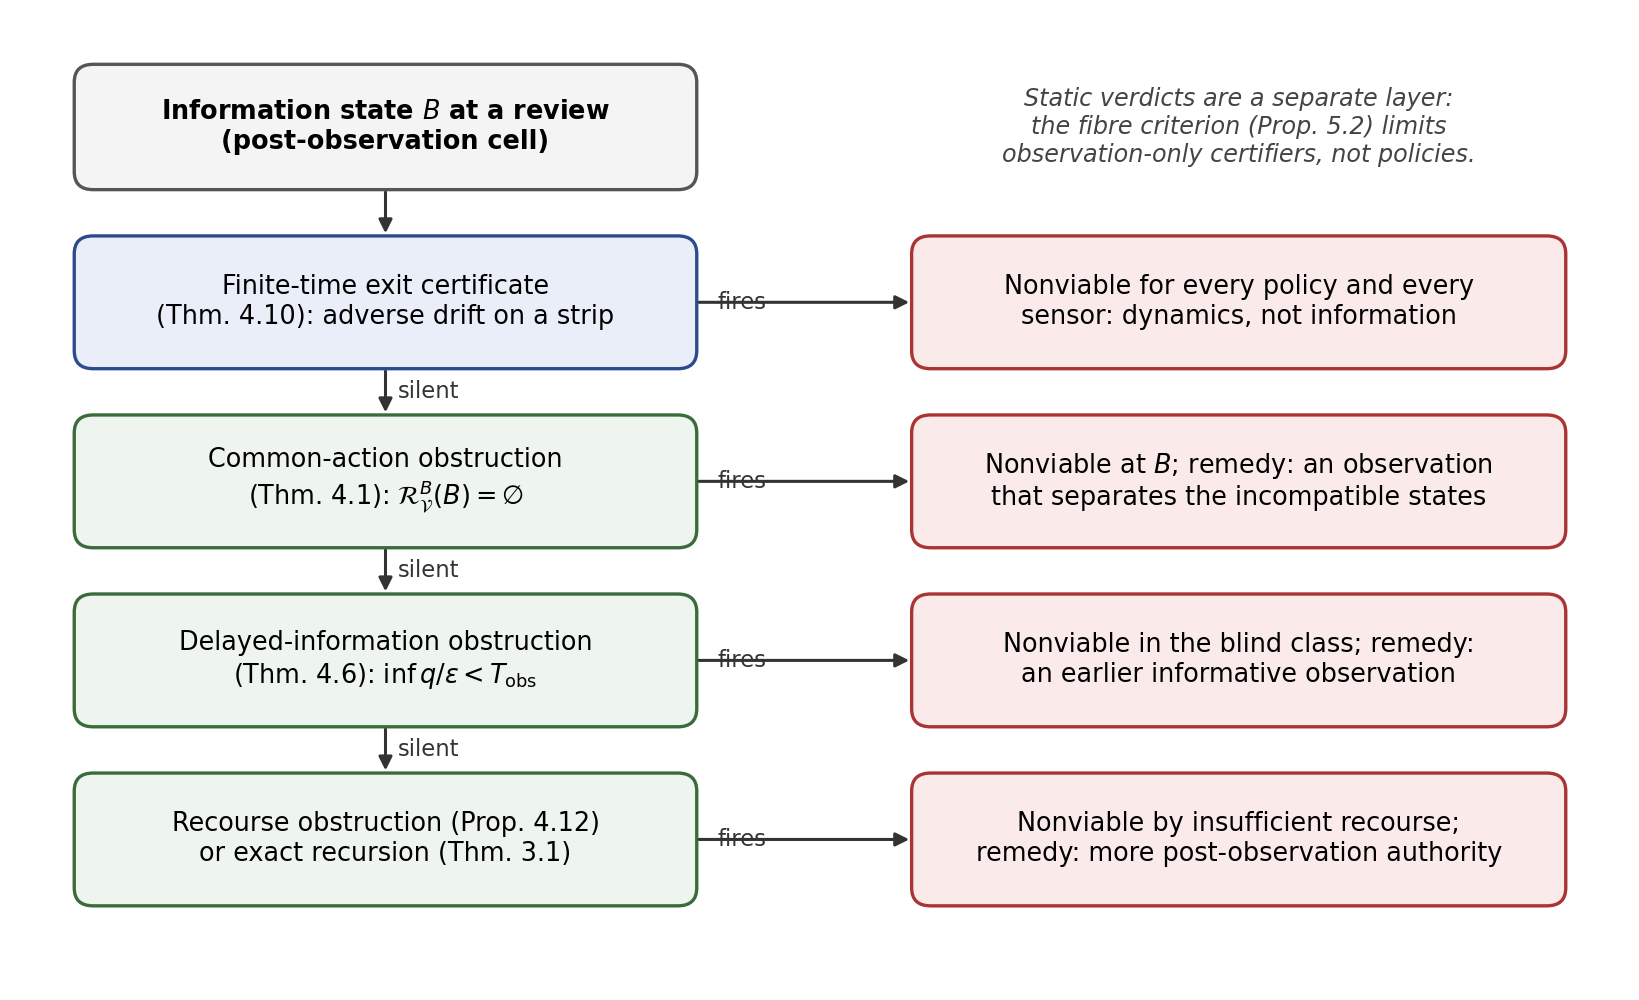
\includegraphics[width=0.9\textwidth]{figs/fig_v73_diagnostic.png}
\caption{The diagnostic use of the calculus at a post-observation information state. Each certificate proves that a specific response correspondence is empty; the mechanism that fires names the design change that could restore the correspondence. The static certification layer (Section~\ref{sec:certification}) constrains verdicts rather than policies and is kept separate.}
\label{fig:diagnostic}
\end{figure}

\subsection{The common-action obstruction}\label{sec:common-action}

The instantaneous obstruction is the static core of the calculus: it certifies nonviability at a single information state without a timing or horizon argument.

\begin{theorem}[common-action obstruction]\label{thm:common-action}
Let $B\subseteq\cV$ be a post-observation information set and consider the held-action review class \hyp{Hold}. Suppose:
\begin{description}[leftmargin=2.6em,itemsep=1pt]
\item[\hyp{C1}] the selected action is held until the next observation;
\item[\hyp{C2}] either $U^B(B)=\varnothing$ (\emph{admissibility obstruction}), or $U^B(B)\ne\varnothing$ and
\begin{equation}\label{eq:common-empty}
\cR^B_\cV(B)=\bigcap_{x\in B}\cR_\cV(x)=\varnothing\qquad\text{(\emph{safety obstruction})};
\end{equation}
\item[\hyp{C3}] (\emph{adverse path, safety case}) for each $a\in U^B(B)$ there exist $x_a\in B\cap\partial\cV$, an active constraint $j_a$, numbers $c_a,\tau_a>0$, and an admissible original-system Carath\'eodory pair $(x_a(\cdot),d_a(\cdot))$ from $x_a$ under the held action $a$, compatible with the pre-review record, with $d_a(t)\in D(x_a(t))$ a.e.\ and $q_{j_a}(x_a(t))\le-c_at<0$ for $0<t<\tau_a$.
\end{description}
Then $B\notin\ERViab_\cI(\cV)$ for the declared class: every compatible state may be individually robustly viable, and the belief is nevertheless nonviable because the state-specific safe actions are incompatible.
\end{theorem}

\begin{proof}
Fix a policy of the class and its held first command $a$. If $a\notin U^B(B)$ it is inadmissible at some compatible state, which is failure by \hyp{Fail}. Otherwise $a\in U^B(B)$, and \eqref{eq:common-empty} says that $a$ fails an active-gradient inequality at some compatible boundary state; \hyp{C3} supplies a realised compatible path from such a state on which the active constraint is strictly negative at arbitrarily small positive times, hence before the next review. The policy was arbitrary within the hold class.
\end{proof}

Hypothesis \hyp{C3} is substantive: a failed gradient test exhibits a disturbance \emph{value} with outward drift, and the certificate needs a disturbance \emph{selection} that realises it along an admissible trajectory. Neither closed graph nor lower semicontinuity of $D$ supplies this (S2.1 gives a closed-graph witness in which a phantom value fails the test while the belief is viable), and a trajectory of the convexified inclusion is not a substitute. The distinction does not make the test less useful---in the polyhedral and finite classes below the path is immediate---but it is what separates a sound certificate from a heuristic.

\paragraph{Farkas form.} When the safe-action constraints over the belief are finitely many affine inequalities $A_iu\le b_i$, stacked as $Au\le b$, the intersection is empty if and only if some $\mu\ge0$ satisfies $\mu^\top A=0$ and $\mu^\top b<0$ \citep{farkas1902,gale1960}: a finite, independently checkable certificate of epistemic infeasibility. Linearity makes the certificate numerically robust---bounded data perturbation degrades the margin $\mu^\top b$ gracefully, and verified approximate multipliers suffice, provided uncertain rows are relaxed toward a \emph{larger} feasible controller set, never a smaller one, since tightening on an unverified worst case can manufacture a false obstruction (S3.1).

\begin{figure}[tb]
\centering
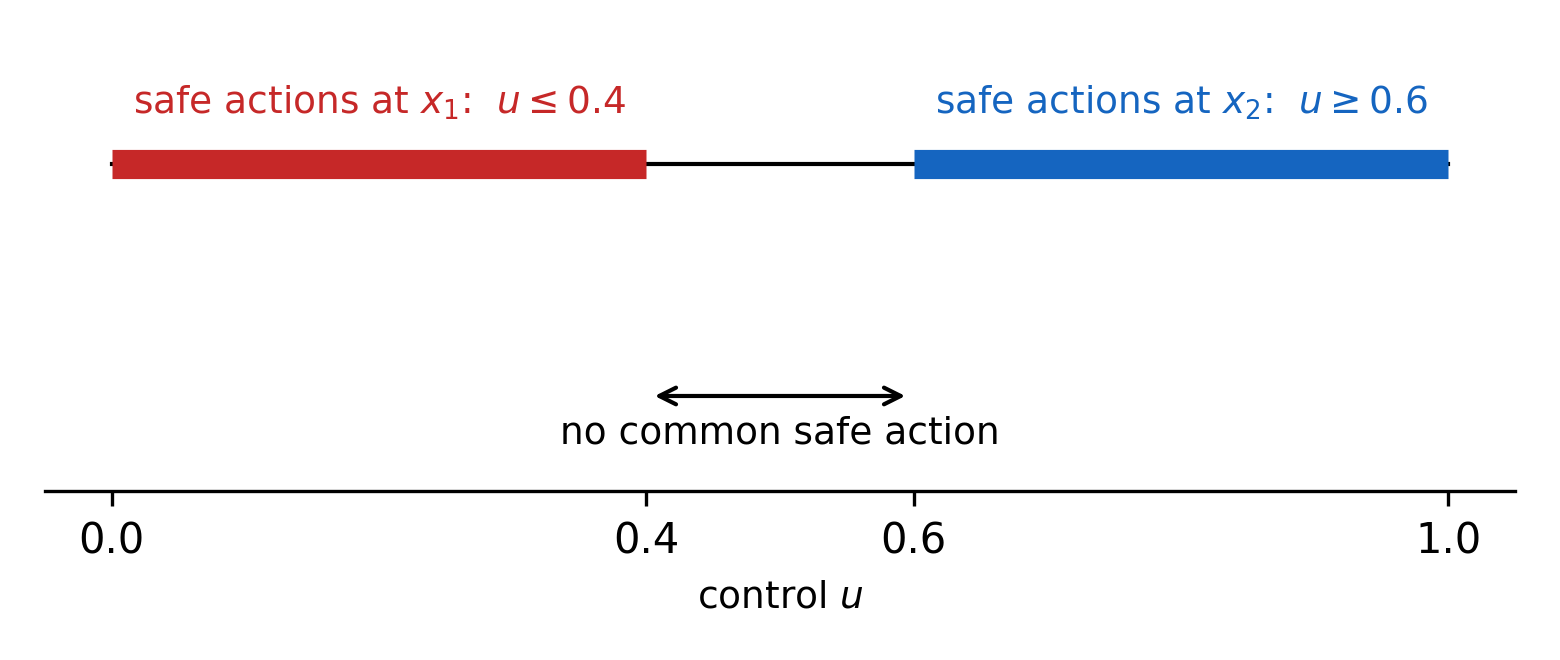
\includegraphics[width=0.6\textwidth]{figs/fig_p2_common_action.png}
\caption{Incompatible safe controls. The states $x_1$ and $x_2$ share an observation but their safe-action sets $[0,0.4]$ and $[0.6,1]$ are disjoint; the Farkas pair $\mu=(\tfrac12,\tfrac12)$ certifies emptiness with margin $0.1$, which shrinks to zero exactly as the two sets come to touch. Any observation separating $x_1$ from $x_2$ restores one-step viability.}
\label{fig:common-action}
\end{figure}

\begin{proposition}[obstruction ladder]\label{prop:ladder}
For the held-action review class, assuming \hyp{C3} at every failed active-gradient test and original-system solutions through the review, the response correspondences are nested,
\[
\Atube(B,\Delta)\;\subseteq\;\cR^B_\cV(B)\;\subseteq\;U^B(B)\qquad(\Delta>0),
\]
and emptiness descends: $U^B(B)=\varnothing\Rightarrow\cR^B_\cV(B)=\varnothing\Rightarrow\Atube(B,\Delta)=\varnothing\Rightarrow B\notin\ERViab_\cI(\cV)$.
\end{proposition}

\begin{proof}
The second inclusion is $\cR_\cV(x)\subseteq U(x)$. For the first, a command in $U^B(B)\setminus\cR^B_\cV(B)$ fails an active-gradient test, and \hyp{C3} supplies an admissible path that exits before every positive review time, so the command is not tube-safe. The last implication is Proposition~\ref{prop:selector}(ii) for policies obliged to hold the first command over this $\Delta$; it says nothing about within-review switching.
\end{proof}

The rungs are strict in general: an instantaneously tangent action may still exit in finite time, which is exactly the gap that \hyp{C3} closes, and the finite recursive correspondence $\cA_N$ joins the ladder only through a sampled-transition model (Figure~S8.1). The dynamic exit certificate of Section~\ref{sec:exit} sits below the ladder: it empties the response set of some compatible state under full information.

\begin{proposition}[sparse common-action witness]\label{prop:helly}
Let $B\subseteq\cV$, let $U\subseteq\R^m$ be compact and convex with $U(x)\subseteq U$ convex and closed, let the dynamics be affine in the control, $f(x,u,d)=f_0(x,d)+f_u(x,d)\,u$, with $D(x)$ compact, and let the $q_j$ be $C^1$. Then each $\cR_\cV(x)$ is a compact convex subset of $U$, and $\bigcap_{x\in B}\cR_\cV(x)=\varnothing$ if and only if it is witnessed by at most $m+1$ compatible states: there are $1\le\ell\le m+1$ states $x_1,\dots,x_\ell\in B$ with $\bigcap_{i\le\ell}\cR_\cV(x_i)=\varnothing$. The admissibility analogue, with $U(x)$ in place of $\cR_\cV(x)$, holds under the same convexity assumptions.
\end{proposition}

\begin{proof}
For fixed $(x,j,d)$ the inequality $\nabla q_j(x)\cdot f(x,u,d)\ge0$ is affine in $u$ and defines a closed half-space, whatever the convexity of $q_j$ in $x$; intersecting over active $j$ and $d\in D(x)$ with the closed convex $U(x)\subseteq U$ gives a compact convex set. If the intersection over $B$ is empty, the finite-intersection property of compact sets yields a finite subfamily with empty intersection, and Helly's theorem in $\R^m$ \citep{helly1923} reduces it to at most $m+1$ members. The converse is immediate.
\end{proof}

\begin{remark}[scope of the count]\label{rem:count}
Convexity is essential: with $U=\R$ and nonconvex safe sets $\{0,1\},\{0,2\},\{1,2\}$ every pair intersects but the triple does not, so no two-state witness exists. The bound also counts \emph{instantaneous} actions, not window-policies. Partition a blind window into $Q$ blocks $I_1,\dots,I_Q$ and let $q+1$ branches be indistinguishable throughout, with scalar input: branch $j\le q$ evolves as $\dot x_j=\mathbf 1_{I_j}(t)(u-1)$ from $x_j(0)=0$ under the floor $x_j\ge0$, forcing $u\equiv1$ on $I_j$, while branch $q+1$ evolves as $\dot x_{q+1}=-u$ from $x_{q+1}(0)=q-\varepsilon$, forcing $\int u\le q-\varepsilon$. The full system is infeasible, yet removing any single branch restores feasibility, so every obstruction involves all $q+1$ branches. For window-policies the governing count is the information--time rank $mQ$, not $m$.
\end{remark}

\begin{proposition}[epistemic emptiness by admissibility: a minimal construction]\label{prop:emptiness}
There is a system with $\Viab(\cV)=\cV\ne\varnothing$ and a non-injective observation $O$ such that every full-fibre initial belief $B_0=O^{-1}(O(S_0))$, $S_0\in\cV$, lies outside $\ERViab_\cI(\cV)$. The mechanism is admissibility: a state-dependent control set leaves a single common action at the merged belief, and that action drifts outward at the boundary.
\end{proposition}

\begin{proof}[Construction]
Take $X=\cV=[1,2]$, $\dot S=u-S$, the unrelaxed nonconvex control sets $U(S)=\{0,S\}$, and the constant observation $O\equiv0$. Under full information $u=S$ gives $\dot S=0$, so every state is viable. Under $O\equiv0$ the only action shared by all $U(S)$ is $0$, so every observation-based policy holds $u=0$ by \hyp{Fail}; then $S(t)=S(0)e^{-t}$ crosses the lower boundary at $t=\log S(0)\le\log2$ and leaves immediately from $S(0)=1$. The construction is Theorem~\ref{thm:common-action}'s safety case at minimal size, with the adverse path explicit; it is epistemic rather than dynamic, since with the constant control set $[0,2]$ in the same plant any $u\equiv m\in(1,2)$ keeps every branch in $[1,2]$. Convexifying the controller sets to $[0,S]$ is a different problem in which $u\equiv1$ is common and safe; no such convexification is used.
\end{proof}

\subsection{The delayed-information obstruction}\label{sec:delayed}

Information may be accurate yet arrive too late. The second certificate turns the timing of the first informative observation into an explicit bound.

\begin{theorem}[delayed-information obstruction]\label{thm:delayed}
Let $B_0\subseteq\cV$ be a compact initial post-observation cell and $\Tobs>0$ a blind horizon. Fix a policy class $\Pi$ of \emph{blind-window controls}: by default all implementable measurable controls on $[0,\Tobs)$, or a declared subclass such as the whole-window hold class. Suppose:
\begin{description}[leftmargin=2.6em,itemsep=1pt]
\item[\hyp{D1}] for each control history in $\Pi$, every compatible realisation produces the same observation record on $[0,\Tobs)$ while safe, so no branch-dependent observation can change the control before exit;
\item[\hyp{D2}] there are a $C^1$ function $q$ on a neighbourhood of the relevant trajectories with $\cV\subseteq\{q\ge0\}$, a number $\varepsilon>0$ and a strip level $a>\max_{B_0}q$ such that, \emph{for every} $u(\cdot)\in\Pi$, there exist a minimiser $x_u\in B_0$ of $q$ and an admissible realisation $d_u(\cdot)$ with an absolutely continuous original-system solution from $x_u$ that follows the common record of \hyp{D1} until exit, exists through any first contact with $q=0$ until it reaches $q<0$ or $\Tobs$, and satisfies, for a.e.\ pre-exit time in the closed strip $0\le q(x(t))\le a$ (boundary contact included),
\begin{equation}\label{eq:drift}
\frac{d}{dt}q(x(t))=\nabla q(x(t))\cdot f(x(t),u(t),d_u(t))\le-\varepsilon;
\end{equation}
\item[\hyp{D3}] the timing bound
\begin{equation}\label{eq:timing}
\Tobs>\frac{\inf_{x\in B_0}q(x)}{\varepsilon}.
\end{equation}
\end{description}
Then no policy of $\Pi$ is viable from $B_0$. For the unrestricted observation-based class this says $B_0\notin\ERViab_\cI(\cV)$; for a proper declared subclass it asserts class-relative nonviability only.
\end{theorem}

\begin{proof}
Fix a policy of $\Pi$. By \hyp{D1} it reduces on $[0,\Tobs)$ to one blind control $u$ (an action inadmissible on a compatible branch already fails). Take the minimiser and realisation of \hyp{D2}, put $h(t)=q(x(t))$, $m=h(0)=\min_{B_0}q\ge0$ and $t_*=m/\varepsilon<\Tobs$, and suppose there is no strict violation by some $t_1\in(t_*,\Tobs)$. As long as $0\le h\le a$, \eqref{eq:drift} integrates to $h(t)\le m-\varepsilon t$; the path cannot first leave the strip through $h=a$, since its derivative is strictly negative there, and at a contact $h=0$ it cannot remain nonnegative, for the same reason. Hence $0\le h(t_1)\le m-\varepsilon t_1<0$, a contradiction. The case $m=0$ is included: negative drift is required \emph{at} the boundary, so contact alone is never mistaken for exit. The quantifier is $\forall\pi\,\exists(x_u,d_u)$; the theorem does not demand that every branch drift downward and need not detect a failure caused only by a non-minimiser branch.
\end{proof}

Condition \eqref{eq:drift} is a condition on the data, not on the policies, and \eqref{eq:timing} is a sufficient timing condition: evading it does not establish viability. Inverted, the bound is a design requirement---the first informative observation must precede the enforced exit time $\inf q/\varepsilon$ (Figure~\ref{fig:timing}). The common-action obstruction is a formal zero-margin counterpart of this certificate, but the two remain distinct: one is a local action-feasibility condition, the other a finite-time survival condition, and they are not related as a $\Tobs\to\infty$ limit (S2.5).

\begin{figure}[tb]
\centering
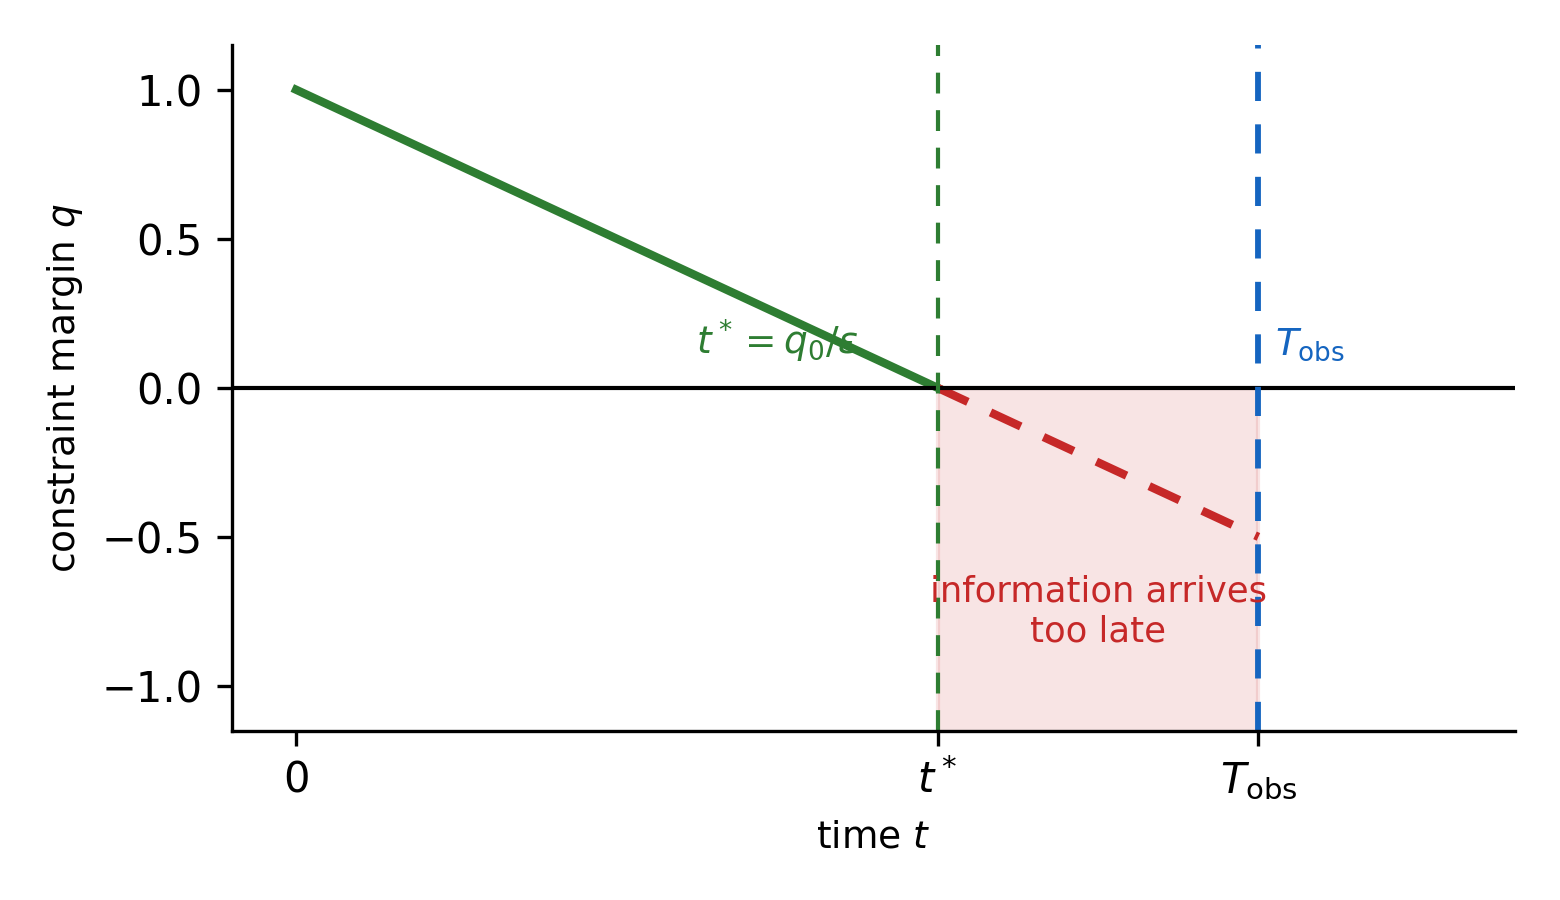
\includegraphics[width=0.58\textwidth]{figs/fig_p2_timing.png}
\caption{Delayed information. Under the compatible adverse-path hypothesis a still-safe branch reaches $q=0$ by $t^*=q_0/\varepsilon<\Tobs$, and continuing the adverse path while it remains safe forces strict exit before the first informative observation (Theorem~\ref{thm:delayed}). The bound need not equal the first contact time.}
\label{fig:timing}
\end{figure}

\begin{remark}[threshold form]\label{rem:sigma}
For a declared blind-window class $\Pi$ let the \emph{guaranteed survival time} be
\[
\sigma^*_\Pi(B_0)=\sup_{u(\cdot)\in\Pi}\ \inf_{x_0\in B_0,\ d(\cdot)}\tau(x_0,u,d),
\]
the infimum over branches that remain observation-equivalent on $[0,\Tobs)$ and $\tau$ the first violation time. Then $\sigma^*_\Pi(B_0)<\Tobs$ implies that no policy of $\Pi$ is viable from $B_0$, because before $\Tobs$ no policy can condition its action on which branch realises. Under \hyp{D1}--\hyp{D2}, for every control in $\Pi$ some branch exits by $\inf q/\varepsilon$, so $\sigma^*_\Pi(B_0)\le\inf q/\varepsilon$ and \eqref{eq:timing} certifies the threshold; the threshold may be strictly smaller, in which case nonviability holds even when \eqref{eq:timing} fails. Emptiness of this blind-window response correspondence is the timing analogue of the tube and common-action rungs.
\end{remark}

For finite blind-window classes (finite $B_0$, hold-until-$\Tobs$ controls from a finite set, or piecewise-constant controls on a finite partition) the drift hypothesis is checked by enumeration of controls together with, for each, an admissible adverse solution with the closed-strip property; enumeration alone does not supply the continuous realisation. Over polytope-declared classes the check is exact and finite.

\begin{theorem}[linear-programming instantiation]\label{thm:lp}
Let the blind window have $K$ discrete steps and finitely many branches $j\in J$ with robust affine dynamics $x^+=A_jx+B_ju+E_jw$, $w\in W_j$ a polytope, known initial branch states $x_{j,0}$, polyhedral safe set $\cV=\{x:Fx\le g\}$, and declared blind-window class $\Pi_B=\{(u_0,\dots,u_{K-1}):u_k\in U\}$ for a polytope $U$. Then:
\begin{enumerate}[label=(\roman*),leftmargin=2.2em,itemsep=1pt]
\item $\sigma^*(B_0;\Pi_B)$ is computed exactly by at most $\lceil\log_2K\rceil+1$ linear programmes of size polynomial in $K$, $|J|$ and the description lengths of $U$, $W_j$, $\cV$; with rational data every step is exact;
\item when the per-step disturbance choices are independent, infeasibility at horizon $K$ is certified by Farkas multipliers---nonnegative weights on the (branch, step, floor) rows whose aggregate control projection vanishes and whose aggregate constant is negative---the timing certificate in adjoint-row form;
\item the programme's feasible set is the declared class itself, so the computation is sound and complete over $\Pi_B$: no relaxation gap arises;
\item the declaration is load-bearing: the per-step polytope programme may be a strict outer relaxation of a separately declared whole-window hold class $\Pi_{\mathrm{hold}}=\{(u,\dots,u):u\in\{-1,+1\}\}$, with a survival gap that grows without bound in $K$.
\end{enumerate}
\end{theorem}

\begin{proof}
Unrolling, $x_{j,k}=A_j^kx_{j,0}+\sum_{i<k}A_j^{k-1-i}(B_ju_i+E_jw_{j,i})$, so for branch $j$, step $k$ and floor row $r$ the robust inequality $F_rx_{j,k}\le g_r$ for all independently selectable $w_{j,i}\in W_j$ is the single linear row
\begin{equation}\label{eq:lprow}
\sum_{i=0}^{k-1}F_rA_j^{k-1-i}B_ju_i\;\le\;g_r-F_rA_j^kx_{j,0}-\sum_{i=0}^{k-1}h_{W_j}\!\bigl(E_j^\top(A_j^{k-1-i})^\top F_r^\top\bigr),
\end{equation}
each support value being a linear programme over $W_j$, precomputed once (for coupled disturbance paths the joint support replaces the sum). The horizon-$K'$ feasibility programme $\{Gu\le b\}$ in $(u_0,\dots,u_{K'-1})$ has one row per (branch, step, floor) plus the rows of $U$; its rows for a shorter horizon are a subset of those for a longer one, so feasibility is monotone and $\sigma^*=\max\{K'\le K:\text{feasible}\}$ is found by bisection, giving (i). Farkas' lemma gives (ii), indexing the multipliers by (branch, step, floor). Claim (iii) is definitional. For (iv) take the non-decaying branches $z^+=z\pm u$ with floor $z\ge1$ from $z_0=2$: either hold survives exactly one blind step, whereas the relaxation $U=[-1,1]$ admits $u\equiv0$, which survives every horizon (S2.6).
\end{proof}

\begin{example}[decaying threshold, and the hold-class gap]\label{ex:relax-gap}
Two branches share $z^+=\tfrac9{10}z\pm u$ from a common $z_0$, floor $z\ge1$, declared class $u_k\in[-1,1]$. The branch sum $z^+_k+z^-_k=2(\tfrac9{10})^kz_0$ is control-invariant, so both floors force $z_0\ge(\tfrac{10}9)^k$ at every step: the window-$K$ programme is feasible exactly when $z_0\ge(\tfrac{10}9)^K$. The level-$k$ Farkas certificate is the pair of floor rows summed---their control coefficients cancel pairwise, the discrete image of pooled adjoint rows---and $u\equiv0$ attains feasibility on the boundary, so the programme is a complete characterisation of this class. The unbounded gap of Theorem~\ref{thm:lp}(iv) concerns a \emph{different}, non-decaying system and a whole-window hold class, and it is specifically a gap between that hold class and its per-step polytope relaxation: in the per-step finite class $\{-1,+1\}^K$ the alternating sequence $+1,-1,+1,\dots$ keeps both branches of $z^+=z\pm u$ safe from any $z_0\ge2$ (verification record, S7).
\end{example}

\subsection{The finite-time exit certificate}\label{sec:exit}

The base obstruction operates before any observation argument: it certifies membership in the full-information ``shadow'' of the kernel \citep{aubin2001,aubin2002}, and when it fires no monitoring design can rescue viability.

\begin{theorem}[finite-time exit certificate]\label{thm:exit}
Let $q:X\to\R$ be $C^1$ with $\cV\subseteq\{q\ge0\}$ and suppose:
\begin{description}[leftmargin=2.6em,itemsep=1pt]
\item[\hyp{E1}] there are $a>0$ and $\varepsilon>0$ such that on the strip $\cS_a=\{x:0\le q(x)\le a\}$
\begin{equation}\label{eq:isaacs}
\sup_{u\in U(x)}\ \inf_{d\in D(x)}D^+q\bigl(x;f(x,u,d)\bigr)\le-\varepsilon\qquad\forall x\in\cS_a;
\end{equation}
\item[\hyp{E2}] (\emph{adverse realisation for the declared control class}) for every admissible control history of the class and every $x_0\in\cS_a$ there is a compatible absolutely continuous original-system trajectory with a measurable disturbance $d(t)\in D(x(t))$, defined beyond $q(x_0)/\varepsilon$ unless it has already reached $q<0$, satisfying $\frac{d}{dt}q(x(t))\le-\varepsilon$ a.e.\ while $0\le q(x(t))\le a$ before exit, and continuing through first contact long enough to decide strict exit.
\end{description}
Then for every control of the declared class and every $x_0\in\cS_a$ an admissible trajectory strictly violates $q\ge0$ before every time strictly greater than $q(x_0)/\varepsilon$; the infimum of strict-violation times is at most $q(x_0)/\varepsilon\le a/\varepsilon$, and viability fails in the class.
\end{theorem}

\begin{proof}
Fix a control and the pair of \hyp{E2}; put $h(t)=q(x(t))$ and $t_0=h(0)/\varepsilon$. If the pair stayed in $\{q\ge0\}$ through some $t_1>t_0$ before its guaranteed continuation ends, it could not first cross upward through $h=a$, and integrating the drift on the still-safe portion gives $0\le h(t_1)\le h(0)-\varepsilon t_1<0$, a contradiction. The drift is never integrated on a path after it has left the strip.
\end{proof}

Condition \eqref{eq:isaacs} has the control-before-disturbance (Isaacs) reading and is information-independent; \hyp{E2} is what makes the pointwise condition a pathwise certificate, and it is a hypothesis about the original game that the standing solution-existence conditions do not discharge (they give a solution for each fixed selection pair, not a drift-consistent adversarial selection coupled to a policy). For an open-loop control one admissible path may depend on the control; disturbance-reactive closed-loop classes need their own compatible-solution premise, for which a state-uniform $d^*$ with $\sup_{u\in U(x)}\nabla q(x)\cdot f(x,u,d^*)\le-\varepsilon$ on the strip is one sufficient condition. A state-dependent barrier may be used with output feedback; only an observation-only barrier subclass must be fibre-constant.

\begin{remark}[comparison-function form]\label{rem:comparison}
If $\dot q\le-\alpha(q)$ with $\alpha:(0,a]\to(0,\infty)$ holds along a compatible adverse trajectory while $q>0$ and $\int_0^{q(x_0)}\dd s/\alpha(s)<\infty$, comparison bounds the time of \emph{first boundary contact}; it does not alone give strict exit from the closed set---the solution of $\dot q=-\sqrt q$ from $q(0)=1$ reaches zero at time two and may stay there. Strict exit requires negative drift at or through contact, as in \hyp{E2}.
\end{remark}

\subsection{The post-observation recourse obstruction}\label{sec:recourse}

The certificates so far fire before information discriminates. The complementary mode---\emph{insufficient post-observation recourse}---is one in which a common blind-window control keeps every branch safe, yet no observation-adapted control can recover every branch once the distinguishing observation arrives. The finite recursion captures it exactly (a four-state instance in which every one-step certificate is silent is S6.3); the following certificate detects it in continuous time for affine systems. It relaxes the post-observation class upward---an oracle grants each stored branch its own controller whether or not the sensor reveals that much---so it is sound but not complete.

\begin{proposition}[oracle-recourse obstruction]\label{prop:recourse}
For each branch $\theta$ and fixed exogenous disturbance scenario $d(\cdot)$ let the dynamics be affine in state and input, $\dot x_\theta=A^d_\theta(t)x_\theta+g^d_\theta(t)+B^d_\theta(t)u$, with bounded measurable coefficients on $[0,T]$ that do not depend on the controlled trajectory; scenarios are exogenous (each admissible $d(\cdot)$ remains admissible under every policy). Let the safety facets be affine, $q_j(x)=c_j^\top x+b_j$ with safety $q_j\ge0$, let $U\subseteq\R^m$ be compact convex, and let branches $x_1,\dots,x_L\in B_0$ be observation-equivalent on $[0,\tau)$ with horizon $T>\tau$. For a label $\ell=(\theta,j,t)$, $t\in(\tau,T]$, let $\bar x^d_\theta$ be the zero-control trajectory, $X^d_\theta(t,\sigma)$ the transition matrix, $\beta^d_\ell=q_j(\bar x^d_\theta(t))$ the zero-control facet margin, and
\[
k^d_\ell(\sigma)=\mathbf 1_{\{\sigma\le t\}}\bigl(B^d_{\theta}(\sigma)\bigr)^\top\bigl(X^d_\theta(t,\sigma)\bigr)^\top\nabla q_j
\]
the input kernel. For weights $\lambda_\ell\ge0$, $\sum_\ell\lambda_\ell=1$, define
\begin{equation}\label{eq:gamma}
\Gamma_h(\lambda)=\inf_{d(\cdot)}\Bigl\{\sum_\ell\lambda_\ell\beta^d_\ell+\int_0^\tau h_U\Bigl(\sum_\ell\lambda_\ell k^d_\ell(\sigma)\Bigr)\dd\sigma+\sum_\ell\int_\tau^Th_U\bigl(\lambda_\ell k^d_\ell(\sigma)\bigr)\dd\sigma\Bigr\}.
\end{equation}
If $\Gamma_h(\lambda)<0$ then $B_0\notin\ERViab_\cI(\cV)$: for every measurable information-adapted policy, at least one stored branch violates a facet under the chosen exogenous scenario (the branch may depend on the policy).
\end{proposition}

\begin{proof}
If the infimum is negative, some exogenous scenario $d^*$ has a negative bracket, and it remains admissible against every policy. For that scenario, variation of constants and affinity of the facets give the \emph{exact} identity $q_j(x^{u,d^*}_\theta(t))=\beta^{d^*}_\ell+\int_0^\tau(k^{d^*}_\ell)^\top w+\int_\tau^t(k^{d^*}_\ell)^\top u_\theta$, where $w$ is the one common window signal (the blind-window reduction of Theorem~\ref{thm:delayed}) and $u_\theta$ the branch's post-reveal signal. Each pairing is bounded above by its support value, so the $\lambda$-weighted facet sum is at most the bracket, hence strictly negative; a strictly negative weighted sum forces some facet strictly negative along its branch. The window signal was arbitrary, so every policy of the class fails (S2.7, including the attainment-special $\phi_U$ variant).
\end{proof}

The state-independent input coefficient and affine facets are load-bearing: for state-dependent $B(x)$ or nonlinear facets the identity is only first-order, and the certificate may fire falsely unless a validated one-sided remainder is added (S2.7 records an explicit scalar counterexample to the control-affine generalisation). Variation of constants evaluates the bracket for a fixed scenario; an admissible scenario with a negative bracket is already a failure witness, whereas a negative lower bound on the infimum is not.

\begin{example}[three branches, delayed recourse]\label{ex:three-branch}
Branches $j=1,2,3$ run the planar double integrator $\dot p=v$, $\dot v=u$ without disturbance from $p_j(0)=\tfrac{34}{25}n_j$, $v_j(0)=n_j$, where $n_1=(1,0)$, $n_2=(-\tfrac35,\tfrac45)$, $n_3=(-\tfrac35,-\tfrac45)$; the actuator set is the hexagon $U=\co\{\pm n_1,\pm n_2,\pm n_3\}$; safety is $n_i^\top p\le2$ for $i=1,2,3$ with $\|v\|_\infty\le\tfrac65$; the realised branch is revealed at time $\tau$. Every branch is viable under full information (brake along $-n_j$ for one second; peak critical position $\tfrac{34}{25}+\tfrac12=\tfrac{93}{50}<2$), and $u\equiv0$ keeps every branch strictly safe through any blind window of length below $\tfrac{16}{25}$, so no instantaneous or blind-window certificate fires. The labels $(j,\,n_j^\top p\le2,\,\tau+1)$ have zero-control margins $\beta_j=\tfrac{16}{25}-\tau-1$ and kernels $\mathbf 1_{\{\sigma\le\tau+1\}}(\tau+1-\sigma)n_j$; the weights $\lambda=(\tfrac38,\tfrac5{16},\tfrac5{16})$ pool the pre-observation kernel to zero, and
\[
\Gamma_h(\tau)=\Bigl(\tfrac{16}{25}-\tau-1\Bigr)+\sum_j\lambda_j\int_\tau^{\tau+1}(\tau+1-\sigma)\dd\sigma=\tfrac7{50}-\tau.
\]
For $\tau>\tfrac7{50}$ the certificate fires and the triple is nonviable---the blind window accumulates braking liability that the post-observation authority cannot discharge on every branch at once---while hold-then-brake is safe exactly to $\tau=\tfrac7{50}$: the threshold is exact. The obstruction is genuinely three-way: at $\tau=\tfrac15$ every pair of branches is jointly viable under a common blind control (worst critical positions $\tfrac{2469}{1250}$ and $\tfrac{2419}{1250}$, Figure~\ref{fig:recourse}), so six of the seven nonempty priors over these branches are viable at a delay where the triple is not; $\Gamma_h(\tfrac15)=-\tfrac3{50}$. All quantities are exact rationals (S3.4, S7).
\end{example}

\begin{figure}[tb]
\centering
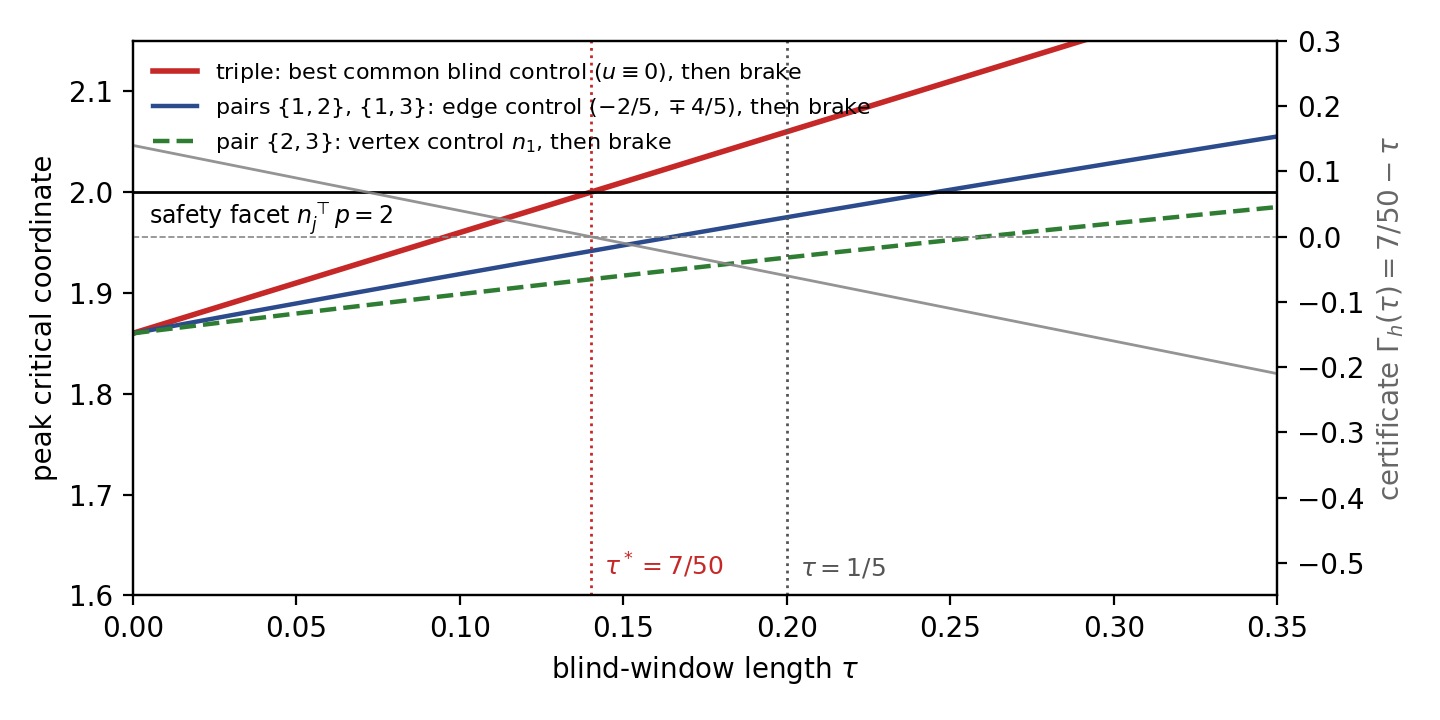
\includegraphics[width=0.8\textwidth]{figs/fig_v73_recourse.png}
\caption{The three-branch recourse instance of Example~\ref{ex:three-branch}. Peak critical coordinate after optimal braking as a function of the blind-window length $\tau$, for the triple under its best common blind control and for the pairs under the stated pair controls; the facet is $2$. The triple fails for $\tau>7/50$, exactly where the certificate $\Gamma_h(\tau)=7/50-\tau$ (grey, right axis) becomes negative, while every pair is still viable at $\tau=1/5$.}
\label{fig:recourse}
\end{figure}
\section{Certification limits}\label{sec:certification}

The certificates of Section~\ref{sec:calculus} concern \emph{policies}. Governance also uses \emph{verdicts}---safe or unsafe---computed from observations alone, without reference to a policy, and the question is when such verdicts can be exact. This is a static classification problem and is kept as a layer separate from viability: a fibre may fail exact certification while a policy is viable, and exact static certification does not imply dynamic viability.

\begin{definition}[exact certifier]\label{def:certifier}
For an admissible domain $Z\subseteq X$ and a safe set $K\subseteq Z$, an \emph{exact certifier} based on $O:Z\to Y$ is a function $C:Y\to\{0,1\}$ with $C(O(z))=1\iff z\in K$ for every $z\in Z$.
\end{definition}

\begin{proposition}[observation-fibre criterion]\label{prop:fibre}
An exact certifier based on $O$ exists if and only if membership in $K$ is constant on every observation fibre,
\begin{equation}\label{eq:fibre}
O(z_1)=O(z_2)\ \Longrightarrow\ \bigl[z_1\in K\iff z_2\in K\bigr]\qquad\forall z_1,z_2\in Z,
\end{equation}
equivalently $K=O^{-1}(O(K))$ on the admissible domain.
\end{proposition}

\begin{proof}
If $C$ exists and $O(z_1)=O(z_2)$ then $\mathbf 1_K(z_1)=C(O(z_1))=C(O(z_2))=\mathbf 1_K(z_2)$. Conversely, \eqref{eq:fibre} makes $C(y)=\mathbf 1_K(z)$ for any $z$ with $O(z)=y$ well defined and exact.
\end{proof}

The criterion applies verbatim to three certification problems that must not be conflated: constraint certification ($K=\cV$), robust-viability certification ($K=\RViab(\cV)$) and policy-specific safety certification ($K=\mathrm{Safe}^\Pi_T$). It is the zero-step, label-valued analogue of the common-action test: an observation-based verdict assigns one label to an entire fibre, exactly as an observation-based action assigns one action to an entire belief, so both are selector problems.

\begin{corollary}[safety-crossing fibres and the certainly-safe set]\label{cor:certainly-safe}
If two admissible states share an observation and one lies in $K$ while the other does not---for an intersection of floors, read $K$ as the single floor $\{q_j\ge0\}$ in question---then no exact observation-only certifier of $K$ exists. The largest set of observations that can soundly be labelled safe without further information is the \emph{certainly-safe set}
\[
\cY_{\mathrm{safe}}=\bigl\{y\in O(Z):\ O^{-1}(y)\subseteq K\bigr\}.
\]
\end{corollary}

\begin{proof}
A fibre meeting both $K$ and its complement violates \eqref{eq:fibre}. On $\cY_{\mathrm{safe}}$ every compatible state is safe, so the verdict ``safe'' is sound; outside it some compatible state is unsafe, so no sound ``safe'' verdict exists.
\end{proof}

A composite index whose fibres cross a floor boundary cannot support exact certification of that floor, however carefully it is thresholded; the certainly-safe set is the region in which the index may certify safety, outside which it must fall silent (Figure~S8.4; worked instances in Section~\ref{sec:casestudy}). The structural requirement is not that each floor be measured separately but that the observation separate every admissible pair lying on opposite sides of the floor; per-floor measurement is one sufficient design.

\paragraph{Bias and the certainty-equivalence trap.} The obstructions above rely on information lost to a non-injective observation. The kernel can also empty under a fully \emph{injective} observation, for a single policy: the canonical certainty-equivalence controller that applies a perfect-information law to the uncorrected observation.

\begin{proposition}[certainty-equivalence trap]\label{prop:ce-trap}
Let $\dot S=u-g(S)$ with $u\in[0,\bar u]$, $g$ continuous and strictly increasing on $[S_{\min},S^*+b]$ with $g(0)=0$, $\cV=[S_{\min},S^*]$, and assume the range condition $g(S+b)\le\bar u$ on $\cV$. Under perfect information the zeroing feedback $u=g(S)$ makes every $S_0\in\cV$ viable. For the injective biased observation $\hat S=S+b$ with $b>0$, the certainty-equivalence controller $u=g(\hat S)=g(S+b)$ gives $\dot S=g(S+b)-g(S)>0$, bounded below by a positive constant on the compact interval, so $S$ exits above $S^*$ in finite time from every $S_0\in\cV$: the kernel of this controller is empty. The bias-corrected controller $u=g(\hat S-b)=g(S)$ restores $\dot S=0$.
\end{proposition}

The mechanism is the failure of one policy to use the observation map's structure, not a loss of information: for a known invertible observation the output-feedback class is as powerful as the state-feedback class, and the statement is policy-specific. No signalling or nonclassical-information phenomenon \citep{witsenhausen1968} is involved.
\section{Completeness and the residual gap}\label{sec:completeness}

The continuous certificates are sufficient conditions, and Section~\ref{sec:finite} showed that in finite systems the pair (common-action test, recursion) is complete. This section locates exactly where completeness can fail in continuous time. Two settings admit an exact answer; the residual gap has a definite structure and is stated as an open problem.

\begin{theorem}[static-observation reduction to open-loop viability]\label{thm:static}
Let $B_0$ be a post-observation cell with one initial reading, $\cV$ compact with $C^1$ constraint functions, $f$ continuous with $D$ compact-valued of closed graph, $U(x)\equiv U$, and let the observation be \emph{static}: $y(t)=O(x(t))$ is constant along every admissible trajectory. Then every observation-based policy coincides with an open-loop control $u(\cdot):[0,\infty)\to U$, and $B_0\in\ERViab_\cI(\cV)$ if and only if some open-loop control keeps every trajectory from every $x_0\in B_0$, under every admissible realisation, in $\cV$ for all time. Within the constant-control subclass $u\equiv u_0$, the robust Nagumo condition \citep{nagumo1942} $\nabla q_j(x)\cdot f(x,u_0,d)\ge0$ for all $x\in\partial\cV$, active $j$ and $d\in D(x)$ is a sufficient test (under the usual tangent-cone and solution-existence regularity) for invariance of $\cV$ from \emph{every} initial state; it is not necessary for viability from a proper subset $B_0$.
\end{theorem}

\begin{proof}
A static observation makes the record constant, so a record-based policy is a time-only control on each initial cell; for a single-reading $B_0$ this is one open-loop control, and the equivalence follows in both directions. The boundary test suffices for invariance of all of $\cV$ under the standard hypotheses, but says nothing necessary about a smaller $B_0$: for $\cV=[0,2]$, $\dot x=x-1$, $B_0=\{1\}$ the stationary trajectory is viable although the velocity is outward at both ends of $\cV$.
\end{proof}

In the static class the obstruction is therefore exactly the nonexistence of a robustly viable open-loop control; a finite obstruction-witness theorem is not supplied for the general static continuous class, and when information accrues, post-observation recourse and timing add distinct modes. The failure of completeness beyond this class has a precise structure. Consider the \emph{two-phase model}: a window of $K$ blind steps with declared blind class $\Pi_B$, followed by a specified reveal.

\begin{proposition}[two-phase decomposition under a typed reveal]\label{prop:decomposition}
Fix a declared blind-window policy class and an exact post-reveal information model. A post-observation cell $B_0$ is viable for the two-phase game if and only if one and the same blind control keeps every compatible branch in $\cV$ through step $K$ \emph{and} places every possible terminal information state in the kernel of the post-reveal policy class---the full-information state kernel under full physical-state revelation, the appropriate post-reveal \emph{belief} kernel when only a branch label is learned and within-branch uncertainty remains.
\end{proposition}

\begin{proof}
Restrict a viable policy to its blind part and then to each possible revealed information state: the blind part is safe and every continuation is viable. Conversely, join a blind witness to a viable continuation after each distinguishable terminal record, which the declared strategy class permits by nonanticipative pasting when the posteriors use the same admissible disturbance histories.
\end{proof}

\begin{proposition}[no window-measurable pair is complete]\label{prop:window-nogo}
Call a certificate pair \emph{window-measurable} when its verdicts depend only on the window sub-model: the initial belief, the branch transitions within the window, the floors and the observation schedule. No window-measurable pair is complete for the two-phase model.
\end{proposition}

\begin{proof}
Take four states with safe set $\{x_1,x_2,x_4\}$, actions $\{a,b\}$, no disturbance, transitions $x_1\colon a\mapsto x_1,\ b\mapsto x_4$; $x_2\colon a\mapsto x_4,\ b\mapsto x_2$; $x_4\colon a,b\mapsto x_3$; initial belief $B_0=\{x_1,x_2\}$, blind at the first step and exactly informed afterwards. The variant changes only $x_4$'s post-reveal transitions to $a,b\mapsto x_4$. All window data coincide, and in both instances every blind action keeps both branches safe through the window, so the common-action and timing certificates are silent. The exact recursion decides differently: in the instance every post-reveal action from $x_4$ exits, so $x_4\notin\RViab(\cV)$ and $B_0\notin\cW_2$ (Proposition~\ref{prop:decomposition} fails on its second clause); in the variant $x_4$ is maintained and $B_0$ is viable. A window-measurable pair returns identical verdicts on the two instances (verification record, S7).
\end{proof}

\begin{proposition}[monotonicity of the epistemic kernel]\label{prop:monotone}
Enlarging the action sets, reducing the disturbance sets, refining the information structure, or enlarging the policy class never shrinks the kernel: for $U_1\subseteq U_2$, $D_1\subseteq D_2$, $\Pi_1\subseteq\Pi_2$ and $\cI_1$ refining $\cI_2$,
\[
\begin{gathered}
\ERViab^{U_1}\subseteq\ERViab^{U_2},\qquad \ERViab^{D_2}\subseteq\ERViab^{D_1},\\
\ERViab^{\Pi_1}\subseteq\ERViab^{\Pi_2},\qquad \ERViab^{\cI_2}\subseteq\ERViab^{\cI_1},
\end{gathered}
\]
the refinement inclusion comparing kernels on the same domain of prior beliefs.
\end{proposition}

\begin{proof}
A policy viable under the smaller action sets, larger disturbance sets, smaller policy class or coarser information remains admissible and nonanticipative under the enlargement or refinement, while the adversary's options are unchanged or reduced; the same policy witnesses viability.
\end{proof}

\begin{openproblem}[dynamic-observation completeness]\label{op:dynamic}
Give a finite, checkable certificate that is necessary and sufficient for membership in $\ERViab_\cI(\cV)$ under dynamic observation, or prove that none exists in a natural class. By Proposition~\ref{prop:window-nogo} any complete pair must read data beyond the window sub-model---the post-observation recourse verdict is the definite target. Abstract transfinite fixed-point recursions do not by themselves provide a finite family of original-system certificates; with exact original-system reachability, disturbance rectangularity, compatible extension and gluing, and implementable measurable belief policies, a belief-space viability kernel gives the matching policy statement, but a generic set-valued reachability recursion need not equal the original policy kernel, and compact reachability and closed observation cells must be supplied if that kernel is formulated on compact beliefs.
\end{openproblem}
\section{A symbolic resource model and a coverage audit}\label{sec:casestudy}

The certificates are now instantiated on a concrete resource model and audited, cell by cell, against the exact recursion of Theorem~\ref{thm:finite-horizon}. The purpose is diagnostic: to show which certificate fires in which regime and what the audit says about the gap between the certificates and the truth. The model is a single-species stock $S\in[0,1]$ (fraction of carrying capacity) with discrete dynamics
\[
S^+=\mathrm{clip}\bigl(S+S(1-S)-u+w\bigr),\qquad u\in[0,0.3],\quad w\in\{-0.02,0,+0.02\},
\]
harvest $u$, recruitment noise $w$ read adversarially, and a sustainability floor $S_{\min}=0.3$ \citep{clark1990}.

\paragraph{Fibre criterion.} The regulator observes a two-bin index, low if $S<0.6$ and high otherwise. The safe set $[0.3,1]$ is not a union of bins---the low bin contains $0.1$ (below the floor) and $0.4$ (above it)---so by Proposition~\ref{prop:fibre} no exact observation-only certifier exists, and by Corollary~\ref{cor:certainly-safe} the certainly-safe set is the single bin $\{\text{high}\}$: a verdict of ``safe'' on a low reading is unsound.

\paragraph{Aggregation in two dimensions.} For a two-species state $(S_1,S_2)\in[0,1]^2$ with floor $S_1\ge0.4$ and an aggregate reading $I=S_1+S_2$, the states $(0.5,0.5)$ and $(0.2,0.8)$ share the reading $I=1.0$ and lie on opposite sides of the floor, so no exact certifier exists; the certainly-safe readings are exactly $I\ge1.4$, since the smallest $S_1$ compatible with $I$ is $I-1$. An aggregate below $1.4$ must fall silent however it is thresholded.

\paragraph{Certainty-equivalence trap.} With $\hat S=S+0.1$, $g(S)=S^2$ and $\cV=[1,2]$ (range condition $\bar u\ge2.1^2$), the uncorrected law $u=g(\hat S)$ gives $\dot S=0.2S+0.01>0$ and reaches the upper bound from $S=1$ in $\approx3.3$ time units, while the corrected law $u=g(\hat S-0.1)$ keeps $\dot S=0$ (Proposition~\ref{prop:ce-trap}).

\paragraph{A delayed hidden-regime model and its policy class.} The state is $(z,\theta)$ with $\theta\in\{-1,+1\}$ unobserved, $z^+=z+\theta u$, $u\in\{-1,+1\}$, floor $z\ge1$; the regime is revealed exactly at the integer horizon $\Tobs$ and not before. The \emph{audited class} is the whole-window hold class $\Pi_{\mathrm{hold}}=\{u_0=\dots=u_{\Tobs-1}\in\{-1,+1\}\}$ with regime-adapted actions after the reveal---an institutional reading in which one management action is fixed for the entire review period. From a known $z_0$ the two held histories after $k<\Tobs$ steps are $z_0\mp k$, so the maximal number of jointly safe blind steps is $\sigma^*_{\mathrm{hold}}(B_0)=\lfloor z_0-1\rfloor$, after the reveal $u=\theta$ restores growth, and viability in the hold class is exactly $z_0\ge1+\Tobs$. The one-step test (Theorem~\ref{thm:onestep}) covers $z_0<2$ (either action sends one regime below the floor at once); the hold-class threshold covers $z_0\ge2$ with $\Tobs>z_0-1$. This is an exact discrete hold-class calculation, not an application of the continuous Theorem~\ref{thm:delayed}; under the broader per-step class the alternating sequence $+1,-1,+1,\dots$ keeps both regimes safe from any $z_0\ge2$ without any observation, so the hold-class verdict does not transfer to it (Theorem~\ref{thm:lp}(iv)). In the fishery above the timing certificate is silent in the normal regime, because $u_0=0$ keeps every stock above the floor.

\begin{table}[tb]
\centering\small
\setlength{\tabcolsep}{4.2pt}
\begin{tabular}{@{}lcccccccccccccccc@{}}
\toprule
$\Tobs$ & \multicolumn{16}{c}{initial position $z_0$}\\
\cmidrule(lr){2-17}
 & 1.0 & 1.1 & 1.2 & 1.3 & 1.4 & 1.5 & 1.6 & 1.7 & 1.8 & 1.9 & 2.0 & 2.1 & 2.2 & 2.3 & 2.4 & 2.5\\
\midrule
1 & $\bullet$ & $\bullet$ & $\bullet$ & $\bullet$ & $\bullet$ & $\bullet$ & $\bullet$ & $\bullet$ & $\bullet$ & $\bullet$ & $\circ$ & $\circ$ & $\circ$ & $\circ$ & $\circ$ & $\circ$\\
2 & $\bullet$ & $\bullet$ & $\bullet$ & $\bullet$ & $\bullet$ & $\bullet$ & $\bullet$ & $\bullet$ & $\bullet$ & $\bullet$ & $\ast$ & $\ast$ & $\ast$ & $\ast$ & $\ast$ & $\ast$\\
3 & $\bullet$ & $\bullet$ & $\bullet$ & $\bullet$ & $\bullet$ & $\bullet$ & $\bullet$ & $\bullet$ & $\bullet$ & $\bullet$ & $\ast$ & $\ast$ & $\ast$ & $\ast$ & $\ast$ & $\ast$\\
\bottomrule
\end{tabular}
\caption{Coverage audit on the delayed hidden-regime model, restricted to one action held throughout the blind window. $\circ$ viable; $\bullet$ nonviable, certified by the one-step common-action test (Theorem~\ref{thm:onestep}); $\ast$ nonviable in the hold class, classified by the discrete hold-class survival threshold and confirmed by exact recursion. All 42 hold-class nonviable cells are covered; the 12 $\ast$ cells are viable under per-step switching.}
\label{tab:coverage}
\end{table}

\paragraph{Coverage audit.} Table~\ref{tab:coverage} and Figure~\ref{fig:coverage} audit the certificates against the exact recursion restricted to the hold class over the grid $z_0\in\{1.0,1.1,\dots,2.5\}$, $\Tobs\in\{1,2,3\}$. Of the 48 cells, 30 are nonviable by the one-step test, 12 are nonviable in the hold class only (later blind step), and 6 are viable. The audit is reproduced in exact rational arithmetic by the verification script (S7).

\begin{remark}[joint completeness in the hold class]\label{rem:coverage}
In the declared hold class the two certificates are jointly complete on this grid: the one-step test covers $z_0<2$, the hold-class threshold covers $2\le z_0<1+\Tobs$, and the two sets partition the 42 nonviable cells exactly. This is completeness in that restricted class only. In the per-step class only the 30 common-action cells are nonviable: the 12 hold-only cells are exactly the cells where in-window adaptivity rescues the declared class, which is the coverage-grid form of the class-declaration clause of Theorem~\ref{thm:lp}.
\end{remark}

\begin{figure}[tb]
\centering
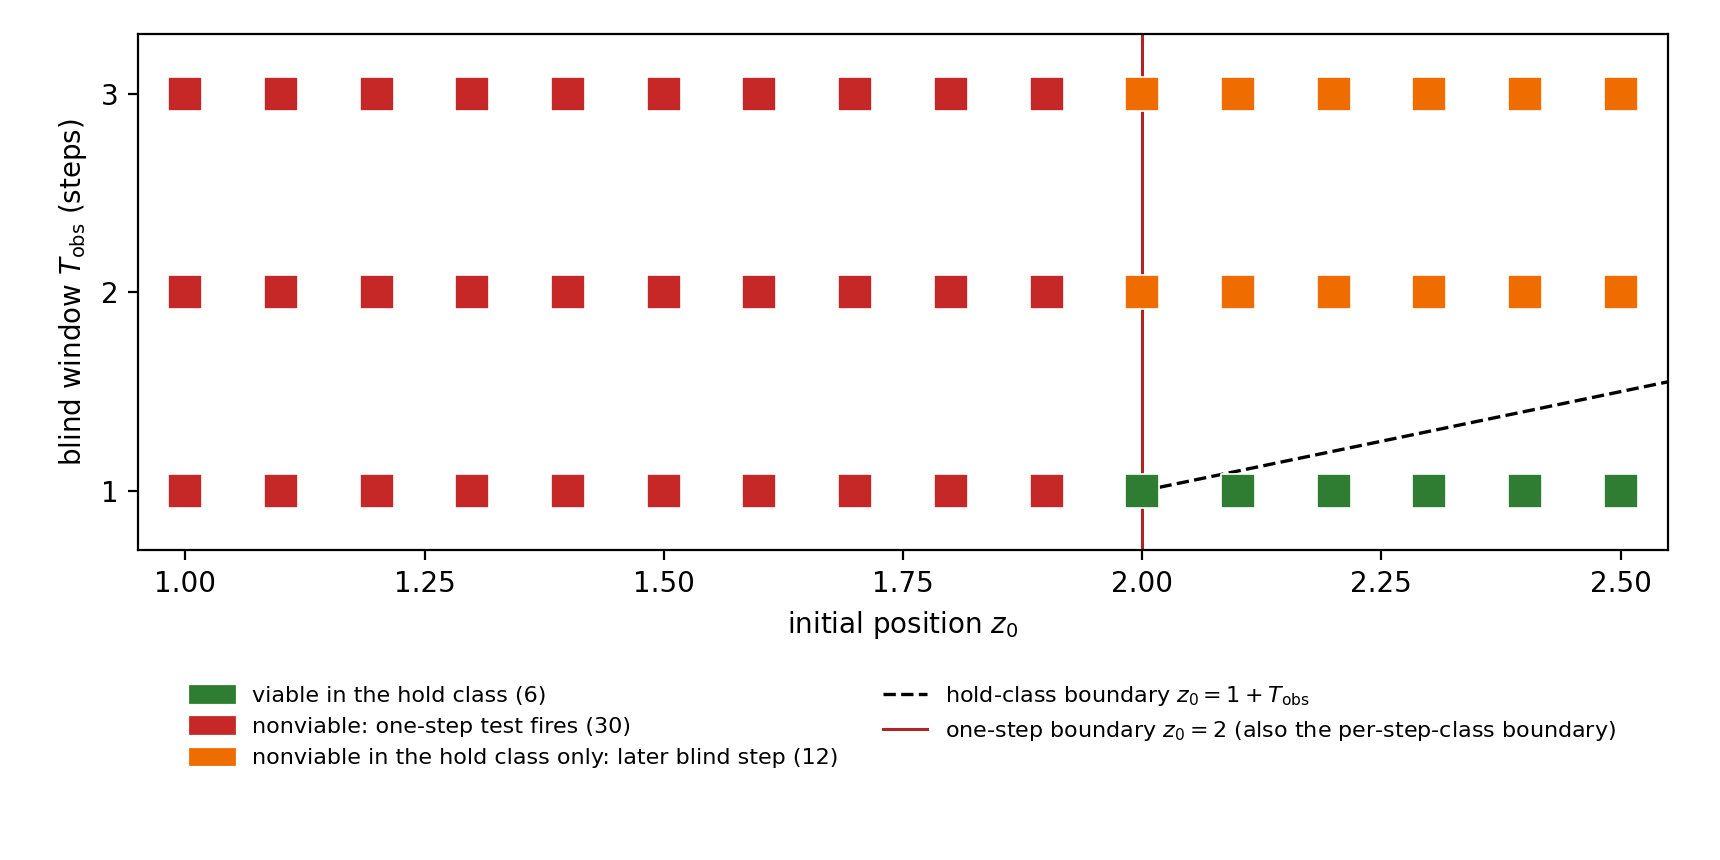
\includegraphics[width=0.98\textwidth]{figs/fig_v73_coverage.png}
\caption{The coverage audit of Table~\ref{tab:coverage}. Green: viable in the hold class; red: nonviable under either class, diagnosed by the one-step test; orange: nonviable only in the audited hold class, established by the discrete hold-class survival calculation. The dashed line is the hold-class boundary $z_0=1+\Tobs$; the solid line $z_0=2$ is both the one-step boundary and the boundary of the per-step class.}
\label{fig:coverage}
\end{figure}

\paragraph{A two-patch protection audit.} At each step one of two patches $z_i\in\{0,1,2,3\}$ receives protection $u\in\{1,2\}$; the transition is $z_i^+=\min\{3,\,z_i+1-2\cdot\mathbf 1[u\ne i]\}$ (the protected patch gains one unit up to the cap, the other loses one net unit), the floor is $z_i\ge1$, and the reading is the aggregate $y=z_1+z_2$. Table~\ref{tab:patch} gives the exact verdicts of the five safe-state fibres. The $y=4$ fibre is the instructive one: all three of its states are safe and individually viable under full information, so $y=4$ is a certainly-safe \emph{reading}, yet the fibre is not viable---action $1$ fails at $(3,1)$ and action $2$ fails at $(1,3)$. The $y=2$ singleton fails even under full information (a dynamic, not an epistemic, failure). The viable $y=5$ fibre has a history-dependent witness: play $u=1$ while the reading stays $5$, reaching the known singleton $(3,1)$ when it first becomes $4$, then alternate $2,1$ to cycle through $(3,1)$ and $(2,2)$. Certainly-safe readings are $y\ge4$; viable full initial fibres have $y\ge5$. The two layers---static verdict and dynamic viability---come apart exactly here.

\begin{table}[tb]
\centering\small
\begin{tabular}{@{}lcll@{}}
\toprule
current fibre & $y$ & verdict & certificate / witness\\
\midrule
$\{(1,1)\}$ & 2 & nonviable & full-information one-step failure\\
$\{(1,2),(2,1)\}$ & 3 & nonviable & no common safe first action (Theorem~\ref{thm:onestep})\\
$\{(1,3),(2,2),(3,1)\}$ & 4 & nonviable & no common safe first action (Theorem~\ref{thm:onestep})\\
$\{(2,3),(3,2)\}$ & 5 & viable & $u=1$ until $y=4$, then $2,1$ cyclically\\
$\{(3,3)\}$ & 6 & viable & $u=1$, then the $y=5$ witness\\
\bottomrule
\end{tabular}
\caption{The five safe-state fibres of the aggregate reading $y=z_1+z_2$ in the two-patch protection model, with exact-recursion verdicts (S7). The $y=4$ reading certifies current safety but supports no common safe action.}
\label{tab:patch}
\end{table}

\paragraph{Calibration.} The certificate parameters correspond to quantities estimable from standard assessment practice: the drift margin $\varepsilon$ is a net growth rate at the floor, the first informative observation time $\Tobs$ is the assessment periodicity, the bias $b$ is the systematic error of the indicator, and the floor is the reference point of the management rule. Calibrating these four numbers from a published assessment is all the machinery the certificates require; the present section stays symbolic and makes no claim of a general-purpose computational calculus for multidimensional belief spaces.
\section{Discussion}\label{sec:discussion}

\subsection{The shape of the calculus}\label{sec:shape}

Table~\ref{tab:summary} collects the certificates, the response correspondence each one empties, and the design consequence each one licenses. The entries are of different kinds and the calculus depends on keeping them apart. The exit certificate is \emph{dynamic}: it defeats every control and needs no observation argument. The common-action obstruction is \emph{static-epistemic}: it defeats every policy of a held-action class at one information state, and Proposition~\ref{prop:emptiness} exhibits it at minimal size. The delayed-information obstruction interpolates between them in time, and the recourse obstruction detects the failure that only appears after information arrives. The fibre criterion limits \emph{verdicts}, not policies, and the certainty-equivalence trap limits one uncorrected policy. The finite recursion supplies the exact counterpart of all of them in finite systems.

\begin{table}[tb]
\centering\small\renewcommand{\arraystretch}{1.1}
\begin{tabularx}{\textwidth}{@{}>{\raggedright\arraybackslash}p{0.36\textwidth}>{\raggedright\arraybackslash}p{0.27\textwidth}X@{}}
\toprule
Certificate & Emptied response correspondence & Design consequence\\
\midrule
finite-time exit (Thm.~\ref{thm:exit}) & response set of some compatible state, under full information & none: dynamics, not information\\\addlinespace[3pt]
common action, admissibility and safety cases (Thm.~\ref{thm:common-action}; Prop.~\ref{prop:emptiness}; ladder, Prop.~\ref{prop:ladder}) & $U^B(B)$, $\cR^B_\cV(B)$, $\Atube(B,\Delta)$ & an observation that separates the incompatible states; a larger common command set\\\addlinespace[3pt]
delayed information (Thm.~\ref{thm:delayed}, Rem.~\ref{rem:sigma}, Thm.~\ref{thm:lp}) & blind-window survival: $\sigma^*_\Pi(B_0)<\Tobs$ & an earlier informative observation\\\addlinespace[3pt]
post-observation recourse (Prop.~\ref{prop:recourse}) & post-reveal continuation (oracle-relaxed) & more post-observation authority; a shorter blind window\\\addlinespace[3pt]
fibre certification (Prop.~\ref{prop:fibre}, Cor.~\ref{cor:certainly-safe}) & exact verdict: $K\ne O^{-1}(O(K))$ & a refined index; per-floor measurement; silence outside $\cY_{\mathrm{safe}}$\\\addlinespace[3pt]
certainty equivalence (Prop.~\ref{prop:ce-trap}) & kernel of the uncorrected controller & correct the known bias\\\addlinespace[3pt]
finite recursion (Thms.~\ref{thm:finite-horizon}, \ref{thm:onestep}) & $B_0\notin\cW_N$ & exact characterisation; obstruction tree\\\addlinespace[3pt]
\bottomrule
\end{tabularx}
\caption{The certificates, the response correspondence each empties, and the design consequence each licenses. The exit, common-action, timing and recourse rows concern nonviability in their stated systems and classes; the fibre row concerns verdicts; the certainty-equivalence row one controller.}
\label{tab:summary}
\end{table}

A failure of observation can thus be \emph{diagnosed} by which certificate applies. If the exit certificate holds, no monitoring design helps. If the common-action obstruction holds, the remedy is an observation that distinguishes the incompatible states, and refinement is never harmful (Proposition~\ref{prop:monotone}), though the theorem claims no benefit beyond removing this test and other mechanisms may still certify nonviability on a finer partition. If the timing bound is violated with slack, the remedy is a shorter review interval or a faster indicator. If the recourse certificate fires, the remedy is authority after the observation rather than information before it. If the fibre criterion fails, the remedy is an observation that separates the sides of the floor rather than a better threshold on the aggregate. In the one-step exact class the design converse is immediate: an observation structure is \emph{adequate} on a target exactly when every fibre meeting the target has a nonempty common safe action---a discrete common-action test, distinct from the static fibre criterion, for which pairwise intersection is necessary and, off convexity, not sufficient (Remark~\ref{rem:count}).

\subsection{Position relative to barrier certificates, estimation tubes and reachability}\label{sec:position}

Barrier certificates certify safety from a scalar function whose zero level set separates the unsafe region from all trajectories \citep{prajna2004,prajna2007}, with a converse under convex-duality conditions \citep{prajna2005} and necessary-and-sufficient hybrid characterisations \citep{maghenem2019}. Theorem~\ref{thm:exit} is the unsafety complement of that converse: a Dini-drift certificate of unsafety that needs no observation structure and is constructive in the enforcing disturbance and exit time. The remaining certificates act at the level of the information set, which barrier constructions---presupposing a state or a specified estimate for feedback---do not address: a search restricted to observation-only barriers is inconclusive about the existence of a common safe action, and a state-dependent barrier need not be constant on fibres merely because the controller is output-based.

The estimation-tube programme carries imperfect measurement to set-valued dynamics on an estimation space \citep{kurzhanski1997,cardaliaguet2007}. Where the reduction applies with matching policy and admissibility hypotheses it is exact for values, and its belief-state controls are common controls. The present theorems delimit its reach rather than contradict it: the obstruction calculus is the local certificate layer of that programme---the common-action obstruction certifies that the belief-state predecessor is empty, the timing bound quantifies when it fails for reasons of information arrival, the fibre criterion says when no observation-based verdict can be exact. Belief-space viability answers \emph{whether}; the obstruction calculus answers \emph{why not, and what to change}. A single worked system carrying the three methods side by side is in S3.5, and the expanded review of the sufficiency results against which the calculus is defined (Veliov's condition, the estimation-tube reduction, observer-and-buffer transfer, and the linear substitution alternative) is S5.

Hamilton--Jacobi reachability \citep{mitchell2005,margellos2011,bansal2017} indexes its value by a physical state and is, like viability theory proper, a sufficiency machine; even under perfect observation its grid solvers scale exponentially in the state dimension, and the learning-based solvers that lift that bound \citep{bansal2021} purchase scalability with approximation. The explicitly finite and polyhedral certificates here address a different verification task---record-constrained set-membership viability---and nothing is claimed about partial-observation reachability methods with their own information-state formulations \citep{chatterjee2009}.

\paragraph{Probabilistic counterpart.} The information-state semantics of this paper is set-membership. Under a stochastic transition and observation likelihood on finite spaces, the maximal survival probability $V_k(b)$ obeys the Smallwood--Sondik belief recursion with an absorbing unsafe state, and the common-action obstruction has a chance-constrained form: if every action loses at least mass $\delta$ from the belief in one step, then $V_k(b)\le1-\delta$ for every $k\ge1$ and the chance constraint at level $1-\varepsilon$ is infeasible for $\varepsilon<\delta$. In the deterministic-kernel limit (single-successor transitions and deterministic observations) $V_k(b)=1$ exactly when $\supp(b)\in\cW_k$, with a deficit of at least the smallest compatible mass otherwise; this bound does not follow from support equality for a genuinely stochastic kernel, which is governed by its transition probabilities. Statements, proofs, the worked instances and the hold-class value table of the audit grid are in S4.

\subsection{Consequences for monitoring and indicator design}\label{sec:design}

Five consequences follow for the design of monitoring in sustainability governance; each is class-relative where its certificate is.

\emph{Timing.} Theorem~\ref{thm:delayed} gives a conditional sufficient bound, not a general minimum frequency: to avoid this failure test the informative observation cannot arrive strictly after $\inf q/\varepsilon$, the worst-case time from the most-constrained compatible state to violation, and an earlier reading is not by itself a viability guarantee. The bound is computable from the drift estimate that a robustness analysis computes in any case.

\emph{Coarseness.} Theorem~\ref{thm:common-action} says that an indicator is exposed when some observation fibre crosses the safe-control partition of the state space. The observation must separate safety classes, not states; keeping every fibre within one class removes this exposure.

\emph{Aggregation.} Proposition~\ref{prop:fibre} applies verbatim to composite indices. An index whose fibres cross a floor cannot support exact floor certification; the certainly-safe set is the domain in which an index-based verdict is sound. The requirement is sharpest where the floor constrains the productive base rather than its output, since an aggregate of services can read at full level while the base regenerating them is reduced beneath it. This is a formal complement to the thesis, argued informally since \citet{martinezalier1998}, that weakly comparable values cannot be fused into one metric without loss; the quantifier-order separation between scalarised and coordinate-wise feasibility that underlies it is developed in \citet{abaee2026aggregate}.

\emph{Bias.} Proposition~\ref{prop:ce-trap} shows that monitoring has two obligations---bounding the observation error and supplying the correction---and that the second lies entirely at the governance structure's discretion: the indicator is published, the correction is not applied, and the safety set of that one uncorrected law empties although a corrected policy remains viable. The remedy is structural correction of the observation map, not a better sensor.

\emph{Institutions.} The hierarchy \eqref{eq:hierarchy} records that epistemic contraction is one of three causes of kernel shrinkage, the others being disturbances and institutional restriction. The institutional kernel $\IRViab_\cJ(\cV)$ combines them: an institution restricted in what it may observe \emph{and} in what it may command inherits both contractions. The certificates remain valid, and typically tighten, when the command set is further restricted, since restriction of the action correspondence can only empty kernels (Proposition~\ref{prop:monotone}). These are design conclusions from the certificates, not empirical findings; their empirical testing belongs to applied studies.

A caution on sensor models: no universal numerical sensor is posited. Thresholded and tolerance-band readings can each fail closed-posterior or approximation obligations under their exact conventions, and any regular-observation lemma must verify joint approximation of reachable states, admissible actions, readings and exact posteriors rather than infer posterior regularity from continuity of the raw sensor.

\subsection{Limitations}\label{sec:limitations}

(i) The continuous-time certificates are sufficient conditions; completeness is claimed only where backward recursion is exact (Section~\ref{sec:finite}) and in the static class (Theorem~\ref{thm:static}). The middle ground---neither a Veliov-type condition nor an obstruction certificate---is open, and continuous completeness would additionally require a measurable-selection theory beyond the explicit selections the certificates exhibit \citep{bertsekas1978}. (ii) The timing obstruction is blind to the recourse mode; the recourse certificate covers it soundly in the affine class under an oracle relaxation, and a complete continuous-time characterisation without that relaxation is open (Open Problem~\ref{op:dynamic}). (iii) The analytic certificates rest on explicit adverse-path hypotheses (\hyp{C3}, \hyp{D2}, \hyp{E2}); when such a premise is unverified the certificate does not certify the model in question, and neither closed graph nor lower semicontinuity of $D$ supplies it. (iv) The semantics is set-membership; the probabilistic counterpart is separate (S4). (v) The examples are finite-dimensional; delay systems require the retarded extension of the comparison argument \citep{hale1993}, and observation error and hidden parameters require their own information models.
\section{Conclusion}\label{sec:conclusion}

The viability literature under incomplete observation has been asymmetric: the sufficiency side is carried by Veliov's condition, the estimation-tube reduction and barrier certificates, while the obstruction side---why a given observation structure cannot sustain a given constraint set---has had no comparable apparatus. This paper supplies that apparatus as a calculus of certificates and shows that it is organised by a single principle: an observation-based regulator must select one response for an entire information state, and each certificate proves that the relevant selection set is empty. In finite systems the principle is exact, through a backward recursion whose one-step case is the common-action test and whose obstruction tree is a finite, mechanically checked witness. In continuous time it yields a ladder of common-action tests with a polyhedral Farkas dual, a timing bound with an explicit slack, an LP relaxation whose gap is identified with the difference between the declared and the per-step policy class, a drift certificate of finite-time exit, and a recourse certificate for the failure that appears only after information arrives. The certification layer adds the fibre criterion and the certainly-safe set as the exact limits of observation-only verdicts, and the certainty-equivalence trap as the one failure that occurs under injective observation.

Three features of the calculus are intended to be used rather than admired. Each certificate names the policy class and the adverse-path hypothesis under which it holds, so that a verdict can be traced to what it assumes. Each certificate names the response correspondence it empties, so that the failure it certifies carries its own remedy. And the gap between the certificates and the truth is located: the certificates are complete in finite systems and in the static class, jointly complete on the audited hold class, and provably incomplete as any window-measurable pair in the two-phase model. The remaining problem---a finite, checkable characterisation of information-state viability under dynamic observation---is stated with the post-observation recourse verdict as its definite target.

For monitoring and indicator design in sustainability governance the message is concrete. An observation structure must separate safety classes, not merely states; it must deliver its first informative reading within a time computable from the drift at the floor; an aggregate index can certify a floor only on its certainly-safe set and must otherwise fall silent; a known bias must be corrected inside the control law, not merely bounded; and when information arrives too late to matter, the design variable is authority after the observation rather than resolution before it. These are theorems about what no design can do, and that is the part of the design problem that has been missing.
\section*{Supplementary material}
\addcontentsline{toc}{section}{Supplementary material}
The Supplementary Material contains: S1 conventions and the concordance with the previous edition; S2 complete proofs of all main-text results, including the selector principle and its phantom-value witness, the obstruction-tree witness, the common-action and delayed-information proofs with their adverse-path hypotheses, the LP gap and the recourse proof with its control-affine counterexample; S3 worked certificates, including the Farkas robustness computation, the three-branch recourse computation and a single system carried through the three methods; S4 the probabilistic counterpart; S5 the sufficiency landscape; S6 the discrete constructions behind the window no-go, the LP gap and the four-state recourse witness; S7 the mechanisation record and the exact-arithmetic verification record V1--V12; S8 additional figures; S9 a map from every main-text result to its proof and verification.

\section*{Declarations}
\paragraph{Funding} None.
\paragraph{Competing interests} None.
\paragraph{Data availability} No external data were used; every numerical value in the paper is derived from the stated symbolic models.
\paragraph{Code availability} The Lean~4 development \texttt{P1\_Obstruction.lean} (Mathlib pin recorded in S7), the exact-arithmetic verification script \texttt{paper01\_v73\_verification.py} (checks V1--V12), the figure script and the discrete coverage runner are distributed with the Supplementary Material and in the public repository \url{https://github.com/MIKEAA2020/general-sustainability}. The coverage runner reproduces the 48-cell hold-class classification of Table~\ref{tab:coverage}; it is a discrete computation, not a continuous-time proof.
\paragraph{Use of AI tools} Large language models (GLM, Z.ai; Qwen, Alibaba Cloud; DeepSeek; and Arena.ai agents) assisted with drafting, restructuring and iterative review. The author reviewed and edited all outputs, verified every mathematical statement, and takes full responsibility for the final work.
\paragraph{Author contributions} A.A. conceived the work, proved the results, and wrote, reviewed and edited the manuscript.

\renewcommand{\refname}{References}
\begin{thebibliography}{99}
\small
\bibitem[Abaee(2026a)]{abaee2026aggregate} Abaee, A.: Aggregate indices and transition safety: a quantifier-order separation between scalarized and coordinate-wise feasibility. figshare, \url{https://doi.org/10.6084/m9.figshare.33764023} (2026)
\bibitem[Abaee(2026b)]{abaee2026preprint} Abaee, A.: An obstruction calculus for viability under incomplete observation. Zenodo, \url{https://doi.org/10.5281/zenodo.22552616}; figshare, \url{https://doi.org/10.6084/m9.figshare.33716593.v2} (2026)
\bibitem[Abaee(2026c)]{abaee2026fish} Abaee, A.: Robust viability of the 2J3KL limit reference point under a surplus-production map: policy scoring, expansion, and when catch cannot help. Zenodo, \url{https://doi.org/10.5281/zenodo.22552060} (2026)
\bibitem[Abaee(2026d)]{abaee2026minimax} Abaee, A.: Minimax dual certificates for the common-action obstruction. Manuscript (2026)
\bibitem[Alshiekh et~al.(2018)]{alshiekh2018} Alshiekh, M., Bloem, R., Ehlers, R., K\"onighofer, B., Niekum, S., Topcu, U.: Safe reinforcement learning via shielding. Proc. AAAI Conf. Artif. Intell. \textbf{32}(1) (2018)
\bibitem[\r{A}str\"om(1965)]{astrom1965} \r{A}str\"om, K.J.: Optimal control of Markov processes with incomplete state information. J. Math. Anal. Appl. \textbf{10}, 174--205 (1965)
\bibitem[Aubin(1991)]{aubin1991} Aubin, J.-P.: Viability Theory. Birkh\"auser, Boston (1991)
\bibitem[Aubin(2001)]{aubin2001} Aubin, J.-P.: Viability kernels and capture basins of sets under differential inclusions. SIAM J. Control Optim. \textbf{40}(3), 853--871 (2001)
\bibitem[Aubin and Catt\'e(2002)]{aubin2002} Aubin, J.-P., Catt\'e, F.: Bilateral fixed-points and algebraic properties of viability kernels and capture basins of sets. Set-Valued Anal. \textbf{10}, 379--416 (2002)
\bibitem[Aubin and Frankowska(1990)]{aubinfrankowska1990} Aubin, J.-P., Frankowska, H.: Set-Valued Analysis. Birkh\"auser, Boston (1990)
\bibitem[Aubin et~al.(2011)]{aubin2011} Aubin, J.-P., Bayen, A.M., Saint-Pierre, P.: Viability Theory: New Directions, 2nd edn. Birkh\"auser, Boston (2011)
\bibitem[Bansal et~al.(2017)]{bansal2017} Bansal, S., Chen, M., Herbert, S.L., Tomlin, C.J.: Hamilton--Jacobi reachability: a brief overview and recent advances. In: Proc. 56th IEEE Conf. Decision and Control (CDC), pp.~2242--2253 (2017)
\bibitem[Bansal and Tomlin(2021)]{bansal2021} Bansal, S., Tomlin, C.J.: DeepReach: a deep learning approach to high-dimensional reachability. In: Proc. IEEE Int. Conf. Robotics and Automation (ICRA), pp.~1817--1824 (2021)
\bibitem[B\'en\'e et~al.(2001)]{bene2001} B\'en\'e, C., Doyen, L., Gabay, D.: A viability analysis for a bio-economic model. Ecol. Econ. \textbf{36}, 385--396 (2001)
\bibitem[Bertsekas and Shreve(1978)]{bertsekas1978} Bertsekas, D.P., Shreve, S.E.: Stochastic Optimal Control: The Discrete-Time Case. Academic Press, New York (1978)
\bibitem[Cardaliaguet et~al.(2007)]{cardaliaguet2007} Cardaliaguet, P., Quincampoix, M., Saint-Pierre, P.: Differential games through viability theory: old and recent results. In: J{\o}rgensen, S., Quincampoix, M., Vincent, T.L. (eds.) Advances in Dynamic Game Theory. Annals of the International Society of Dynamic Games, vol.~9, pp.~3--35. Birkh\"auser, Boston (2007)
\bibitem[Chatterjee et~al.(2009)]{chatterjee2009} Chatterjee, K., Doyen, L., Henzinger, T.A.: Qualitative analysis of partially-observable Markov decision processes. In: Mathematical Foundations of Computer Science (MFCS 2009). LNCS, vol.~5734, pp.~635--646. Springer, Berlin (2009)
\bibitem[Clark(1990)]{clark1990} Clark, C.W.: Mathematical Bioeconomics: The Optimal Management of Renewable Resources, 2nd edn. Wiley, New York (1990)
\bibitem[Crandall et~al.(1992)]{crandall1992} Crandall, M.G., Ishii, H., Lions, P.-L.: User's guide to viscosity solutions of second order partial differential equations. Bull. Amer. Math. Soc. (N.S.) \textbf{27}, 1--67 (1992)
\bibitem[De Lara and Doyen(2008)]{delara2008} De Lara, M., Doyen, L.: Sustainable Management of Natural Resources: Mathematical Models and Methods. Springer, Berlin (2008)
\bibitem[Doyen(2000)]{doyen2000} Doyen, L.: Guaranteed output feedback control for uncertain systems under control and state constraints. Set-Valued Anal. \textbf{8}, 149--162 (2000)
\bibitem[Doyen and Gajardo(2020)]{doyen2020} Doyen, L., Gajardo, P.: Sustainability standards, multicriteria maximin, and viability. Nat. Resour. Model. \textbf{33}(3), e12250 (2020)
\bibitem[Doyen et~al.(2012)]{doyen2012} Doyen, L., Th\'ebaud, O., B\'en\'e, C., Martinet, V., Gourguet, S., Bertignac, M., Fifas, S., Blanchard, F.: A stochastic viability approach to ecosystem-based fisheries management. Ecol. Econ. \textbf{75}, 32--42 (2012)
\bibitem[Farkas(1902)]{farkas1902} Farkas, J.: Theorie der einfachen Ungleichungen. J. Reine Angew. Math. \textbf{124}, 1--27 (1902)
\bibitem[Frankowska(1989)]{frankowska1989} Frankowska, H.: Optimal trajectories associated with a solution of contingent Hamilton--Jacobi equations. Appl. Math. Optim. \textbf{19}, 291--311 (1989)
\bibitem[Gale(1960)]{gale1960} Gale, D.: The Theory of Linear Economic Models. McGraw-Hill, New York (1960)
\bibitem[Haddad(1981)]{haddad1981} Haddad, G.: Monotone viable trajectories for functional-differential inclusions. J. Differ. Equ. \textbf{42}, 1--24 (1981)
\bibitem[Hale and Verduyn Lunel(1993)]{hale1993} Hale, J.K., Verduyn Lunel, S.M.: Introduction to Functional Differential Equations. Springer, New York (1993)
\bibitem[Helly(1923)]{helly1923} Helly, E.: \"Uber Mengen konvexer K\"orper mit gemeinschaftlichen Punkten. Jahresber. Dtsch. Math.-Ver. \textbf{32}, 175--176 (1923)
\bibitem[Kurzhanski and V\'alyi(1997)]{kurzhanski1997} Kurzhanski, A.B., V\'alyi, I.: Ellipsoidal Calculus for Estimation and Control. Birkh\"auser, Boston (1997)
\bibitem[Maghenem and Sanfelice(2019)]{maghenem2019} Maghenem, M., Sanfelice, R.G.: Characterizations of safety in hybrid inclusions via barrier functions. In: Proc. 22nd ACM Int. Conf. Hybrid Systems: Computation and Control (HSCC), pp.~109--118 (2019)
\bibitem[Margellos and Lygeros(2011)]{margellos2011} Margellos, K., Lygeros, J.: Hamilton--Jacobi formulation for reach--avoid differential games. IEEE Trans. Automat. Control \textbf{56}(8), 1849--1861 (2011)
\bibitem[Martinez-Alier et~al.(1998)]{martinezalier1998} Martinez-Alier, J., Munda, G., O'Neill, J.: Weak comparability of values as a foundation for ecological economics. Ecol. Econ. \textbf{26}(3), 277--286 (1998)
\bibitem[Mitchell et~al.(2005)]{mitchell2005} Mitchell, I.M., Bayen, A.M., Tomlin, C.J.: A time-dependent Hamilton--Jacobi formulation of reachable sets for continuous dynamic games. IEEE Trans. Automat. Control \textbf{50}(7), 947--957 (2005)
\bibitem[Nagumo(1942)]{nagumo1942} Nagumo, M.: \"Uber die Lage der Integralkurven gew\"ohnlicher Differentialgleichungen. Proc. Phys.-Math. Soc. Japan \textbf{24}, 551--559 (1942)
\bibitem[Papadimitriou and Tsitsiklis(1987)]{papadimitriou1987} Papadimitriou, C.H., Tsitsiklis, J.N.: The complexity of Markov decision processes. Math. Oper. Res. \textbf{12}(3), 441--450 (1987)
\bibitem[Prajna and Jadbabaie(2004)]{prajna2004} Prajna, S., Jadbabaie, A.: Safety verification of hybrid systems using barrier certificates. In: Alur, R., Pappas, G.J. (eds.) Hybrid Systems: Computation and Control (HSCC 2004). LNCS, vol.~2993, pp.~477--492. Springer, Berlin (2004)
\bibitem[Prajna et~al.(2007)]{prajna2007} Prajna, S., Jadbabaie, A., Pappas, G.J.: A framework for worst-case and stochastic safety verification using barrier certificates. IEEE Trans. Automat. Control \textbf{52}(8), 1415--1428 (2007)
\bibitem[Prajna and Rantzer(2005)]{prajna2005} Prajna, S., Rantzer, A.: On the necessity of barrier certificates. IFAC Proc. Vol. \textbf{38}(1), 526--531 (2005)
\bibitem[Quincampoix and Veliov(1994)]{quincampoix1994} Quincampoix, M., Veliov, V.M.: Viability with a target: theory and applications. In: Control Theory, Multivariate Analysis and Applications, pp.~47--63. Springer (1994)
\bibitem[Saint-Pierre(1994)]{saintpierre1994} Saint-Pierre, P.: Approximation of the viability kernel. Appl. Math. Optim. \textbf{29}, 187--209 (1994)
\bibitem[Smallwood and Sondik(1973)]{smallwood1973} Smallwood, R.D., Sondik, E.J.: The optimal control of partially observable Markov processes over a finite horizon. Oper. Res. \textbf{21}(5), 1071--1088 (1973)
\bibitem[Veliov(1993)]{veliov1993} Veliov, V.M.: Sufficient conditions for viability under imperfect measurement. Set-Valued Anal. \textbf{1}, 305--317 (1993)
\bibitem[Witsenhausen(1968)]{witsenhausen1968} Witsenhausen, H.S.: A counterexample in stochastic optimum control. SIAM J. Control \textbf{6}(1), 131--147 (1968)
\end{thebibliography}

\end{document}
